\documentclass[russian,utf8,12pt]{eskdtext}
\usepackage[numbertop, numbercenter]{eskdplain}

% - Подключаем шрифты из пакета scalable-cyrfonts-tex
\usepackage{cyrtimes}

% - Отступ красной строки
\setlength{\parindent}{1.25cm}

% - Убирает точку в списке литературы
\makeatletter
\def\@biblabel#1{#1 }

% - Точки для всех пунктов в оглавлении
\renewcommand*{\l@section}{\@dottedtocline{1}{1.5em}{2.3em}}
\renewcommand*{\l@subsection}{\@dottedtocline{1}{1.5em}{2.3em}}
\renewcommand*{\l@subsubsection}{\@dottedtocline{1}{1.5em}{2.3em}}

% - Для переопределения списков
\renewcommand{\theenumi}{\arabic{enumi}}
\renewcommand{\labelenumi}{\theenumi)}
\makeatother

\usepackage{enumitem}
\setlist{nolistsep, itemsep=0.3cm,parsep=0pt}

% - ГОСТ списка литературы
\bibliographystyle{utf8gost705u}

% - Верикальные отступы заголовков 
\ESKDsectSkip{section}{1em}{1em}
\ESKDsectSkip{subsection}{1em}{1em}
\ESKDsectSkip{subsubsection}{1em}{1em}

% - Изменение заголовков
\usepackage{titlesec}
\titleformat{\section}{\centering\normalfont\normalsize}{\thesection}{1.0em}{}
\titleformat{\subsection}{\centering\normalfont\normalsize}{\thesubsection}{1.0em}{}
\titleformat{\subsubsection}{\centering\normalfont\normalsize}{\thesubsubsection}{1.0em}{}
\titleformat{\paragraph}{\centering\normalsize}{\theparagraph}{1.0em}{}

% - Оставим место под ТЗ 
%\setcounter{page}{4}

% - Для больших таблиц
\usepackage{longtable}
\usepackage{tabularx}
\renewcommand{\thetable}{\thesection.\arabic{table}}

% - Используем графику в документе
\usepackage{graphicx}
\graphicspath{{images/}}
\renewcommand{\thefigure}{\thesection.\arabic{figure}}

% - Счётчики
\usepackage{eskdtotal}

% - Выравнивание по ширине
\sloppy

% - Разрешить перенос двух последних букв слова
\righthyphenmin=2

\RequirePackage{enumitem}
\renewcommand{\alph}[1]{\asbuk{#1}}
\setlist{nolistsep}
\setitemize[1]{label=--, fullwidth, itemindent=\parindent, 
  listparindent=\parindent}% для дефисного списка
\setenumerate[1]{label=\arabic*), fullwidth, itemindent=\parindent, 
  listparindent=\parindent}% для нумерованного списка
\setenumerate[2]{label=\alph*), fullwidth, itemindent=\parindent, 
  listparindent=\parindent, leftmargin=\parindent}% для списка 2-ой ступени, который будет нумероваться а), б) и т.д.

\usepackage{listings}  
\lstset{basicstyle=\ttfamily\small}

\begin{document}
 \newpage
\ESKDthisStyle{empty}

\begin{center}
 Министерство образования и науки Российской Федерации\\
 Федеральное государственное бюджетное образовательное учреждение высшего профессионального образования\\
 <<ТОМСКИЙ ГОСУДАРСТВЕННЫЙ УНИВЕРСИТЕТ СИСТЕМ УПРАВЛЕНИЯ И РАДИОЭЛЕКТРОНИКИ>> (ТУСУР)\\
 Кафедра комплексной информационной безопасности электронно-вычислительных систем (КИБЭВС)\\
\end{center}

\vfill

\begin{flushright}
\begin{minipage}{0.45\textwidth}
 \begin{flushleft}
  УТВЕРЖДАЮ\\
  заведующий каф. КИБЭВС
  \underline{\hspace{3cm}}А.А. Шелупанов \\
  <<\underline{\hspace{1cm}}>>\underline{\hspace{3cm}}2016г.\\
 \end{flushleft}
\end{minipage}
\end{flushright}

\vfill

\begin{center}
КОМПЬЮТЕРНАЯ ЭКСПЕРТИЗА

Отчет по групповому проектному обучению

Группа КИБЭВС-1401
\end{center}

\vfill
\begin{flushright}
\begin{minipage}{0.45\textwidth}
 \begin{flushleft}
  Ответственный исполнитель \\
  студент гр. 722 \\
  \underline{\hspace{3cm}}О.В. Лобанов \\
  <<\underline{\hspace{1cm}}>>\underline{\hspace{3cm}}2016г.\\
 \end{flushleft}
\end{minipage}
\end{flushright}

\vfill

\begin{flushright}
\begin{minipage}{0.45\textwidth}
 \begin{flushleft}
  Научный руководитель \\
  аспирант каф. КИБЭВС \\
  \underline{\hspace{3cm}}А.И. Гуляев \\
  <<\underline{\hspace{1cm}}>>\underline{\hspace{3cm}}2016г.\\
 \end{flushleft}
\end{minipage}
\end{flushright}

\vfill

\begin{center}
 2016
\end{center}

 \newpage
\ESKDthisStyle{empty}
\paragraph{\hfill РЕФЕРАТ \textbf{ПРАВИТЬ!!!} \hfill}
Курсовая работа содержит \ESKDtotal{page} страниц, \ESKDtotal{figure} рисунка, \ESKDtotal{table} таблицы, \ESKDtotal{bibitem} источников, \ESKDtotal{appendix} приложение.

%допилить ключевые слова
КОМПЬЮТЕРНАЯ ЭКСПЕРТИЗА, ФОРЕНЗИКА, ЛОГИ, QT, XML, GIT, LATEX, ICQ, MS OUTLOOK, WINDOWS, PST, MSG, RTF, HTML, БИБЛИОТЕКИ, РЕПОЗИТОРИЙ, МЕССЕНДЖЕР, ПОЧТОВЫЙ КЛИЕНТ, SQLLITE, РЕЕСТР, ИЗОБРАЖЕНИЯ, READPST, JPEG, PNG.

Цель работы --- создание программного комплекса, предназначенного для проведения компьютерной экспертизы.

Задачей, поставленной на данный семестр, стало написание программного комплекса, имеющего следующие возможности: 
\begin{enumerate}
\item сбор и анализ информации из реестра;
\item сбор и анализ информации из журналов истории браузеров;
\item сбор и анализ информации из мессенджеров;
\item сбор и анализ информации из почтовых приложений;
\item идентификации файлов изображений по внутреннему содержимому и их проверка;
\item сбора информации об установленном ПО по остаточным файлам.
\end{enumerate}

Результаты работы в данном семестре:

\begin{itemize}
\item реализован алгоритм извлечения строковых переменных из реестра Windows;
\item реализован алгоритм побитового считывания файла формата PST;
\item реализован импорт истории (посещений, поисковых запросов, загруженных файлов), закладок и 
другой информации (версия приложения, логин аккаунта google) из приложения Google Chrome;
\item реализован алгоритм парсинга контактного листа пользователя, сохраняемого приложением ICQ;
\item реализована проверка конца файла для форматов JPEG и PNG (для идентификации файлов изображений) и проверка заголовков 5 форматов изображений;
\end{itemize}

Пояснительная записка выполнена при помощи системы компьютерной вёрстки \LaTeX.

 
 \newpage
 \ESKDthisStyle{empty}
 \section*{Список исполнителей}
 
Кучер М.В. -- программист, ответственный за разработку плагина для извлечения информации о пользовательских аккаунтах в мессенджере Viber.

Мейта М.В. -- программист, документатор, ответственный за доработку архитектуры проекта, а также верстку необходимой документации в системе \LaTeX.

Терещенко Ю.А. -- программист, ответственный за написание плагина для сбора сохраненных логинов и паролей браузера Mozilla Firefox.

Шиповской В.В. -- программист, ответственный за дозработку графического интерфейса пользователя системы <<COEX>> и анализ данных, хранимых в NoSql БД Apache Solr.

Боков И.М. -- программист, ответственный за документирование программных модулей на языке MarkDown.

Лобанов О.В. -- программист, ответственный за разработку сайта <<coex.su>> проекта и плагина PDFChecker. 

Серяков А.В. -- программист, ответственный за сборку пакетов для распространения и установки программного обеспечения <<COEX>>.



 % - содержание
 \newpage
 \ESKDstyle{plain}
 \tableofcontents

 \newpage
 \ESKDstyle{plain}
 \section*{Введение}
 \addcontentsline{toc}{section}{Введение}
 Компьютерно-техническая экспертиза является классом инженерно-\\технических экспертиз, проводимых в целях поиска криминалистически значимой информации на носителях, её всестороннего исследование, и, как следствие, получения доказательственной информации и установления фактов, имеющих значение для уголовных, гражданских и административных дел, сопряжённых с использованием компьютерных технологий. Для проведения компьютерных экспертиз необходима высокая квалификация экспертов, так как при изучении представленных носителей информации, попытке к ним доступа и сбора информации возможно внесение в информационную среду изменений или полная утрата важных данных.

Компьютерная экспертиза, в отличие от компьютерно-технической экспертизы, затрагивает только информационную составляющую, в то время как аппаратная часть и её связь с программной средой не рассматривается.

На протяжении предыдущих семестров нами были рассмотрены такие направления компьютерной экспертизы, как исследование файловых систем, сетевых протоколов, организация работы серверных систем, механизм журналирования событий. Также нами были изучены основные задачи, которые ставятся перед сотрудниками правоохранительных органов, которые проводят компьютерную экспертизу, и набор чуществующих утилит, способных помочь эксперту в проведении компьютерной экспертизы. Было выявлено, что существует множество разрозненных программ, предназначенных для просмотра лог-файлов системы и таких приложений, как мессенджеры и браузеры, но для каждого вида лог-файлов необходимо искать отдельную программу. Так как ни одна из них не позволяет эксперту собрать воедино и просмотреть все логи системы, браузеров и мессенджеров, было решено создать для этой цели собственный автоматизированный комплекс, которому на данный момент нет аналогов.


 \section{Назначение и область применения}
Разрабатываемый комплекс предназначен для автоматизации процесса сбора информации с исследуемого образа жёсткого диска.

\section{Постановка задачи}
\setcounter{figure}{0}
На данный семестр были поставлены следующие задачи:

\begin{itemize}
\item изучение архитектуры проекта <<Компьютерная экспертиза>> новыми участниками проектной группы;
\item изучение теоретического материала и основных инструментов разработки;
\item определение индивидуальных задач для каждого участника проектной группы;
\item исследование предметных областей в рамках индивидуальных задач; 
\item реализация новых программных модулей и доработка уже существующих;
\item изучение инструментов для генерации документации к программному коду проекта.
\end{itemize}

Задачи по проектированию модулей:

\begin{enumerate}
\item сбор и анализ информации из реестра Windows;
\item сбор и анализ информации из браузера Google Chrome;
\item сбор и анализ информации из почтового клиента Mozilla Thunderbird;
\item сбор и анализ информации из почтового клиента MS Outlook;
\item поиск медиа-файлов (аудио, видео, изображение) и извлечение мета-данных из них;
\item сбор информации об установленном ПО по остаточным файлам.
\end{enumerate}


\section{Инструменты}
\setcounter{figure}{0}
\subsection{Система контроля версий Git}
Для разработки программного комплекса для проведения компьютерной экспертизы было решено использовать Git.

Git --- распределённая система управления версиями файлов. Проект был создан Линусом Торвальдсом для управления разработкой ядра Linux  как противоположность  системе управления версиями Subversion (также известная как «SVN»). \cite{progit}

При работе над одним проектом команде разработчикоа необходим инструмент для совместного написания, бэкапирования и тестирования программного обеспечения. Используя Git, мы имеем:
\begin{itemize}
\item возможность удаленной работы с исходными кодами;
\item возможность создавать свои ветки, не мешая при этом другим разработчикам;
\item доступ к последним изменениям в коде, т.к. все исходники хранятся на сервере git.keva.su;
\item исходные коды защищены, доступ к ним можно получить лишь имея RSA-ключ;
\item возможность откатиться к любой стабильной стадии проекта.
\end{itemize}

Основные постулаты работы с кодом в системе Git:

\begin{itemize}
\item каждая задача решается в своей ветке;
\item необходимо делать коммит как только был получен осмысленный результат;
\item ветка master мержится не разработчиком, а вторым человеком, который производит вычитку и тестирование изменения;
\item все коммиты должны быть осмысленно подписаны/прокомментированы.
\end{itemize}


\subsection{Система компьютерной вёрстки \TeX}
\TeX\ --- это созданная американским математиком и программистом Дональдом Кнутом система для вёрстки текстов. Сам по себе \TeX\ представляет собой специализированный язык программирования.Каждая издательская система представляет собой пакет макроопределений этого языка.

\LaTeX\ --- это созданная Лэсли Лэмпортом издательская система на базе \TeX'а \cite{lvovskyi} \LaTeX\ позволяет пользователю сконцентрировать свои услия на содержании и структуре текста, не заботясь о деталях его оформления.

Для подготовки отчётной и иной документации нами был выбран \LaTeX\, так как совместно с системой контроля версий Git он предоставляет возможность совместного создания и редактирования документов. Огромным достоинством системы \LaTeX\ то, что создаваемые с её помощью файлы обладают высокой степенью переносимости. \cite{latexrus}

Совместно с \LaTeX\ часто используется Bib\TeX\ --- программное обеспечение для создания форматированных списков библиографии. Оно входит в состав дистрибутива \LaTeX\ и позволяет создавать удобную, универсальную и долговечную библиографию. Bib\TeX\ стал одной из причин, по которой нами был выбран \LaTeX\ для создания документации.

\subsection{Язык разметки Markdown}
Markdown — это язык форматирования (или язык описания форматирования), по принципу работы похожий на HTML, который используется для определения финального вида текста.
Работает это следующим образом — в текстовое поле вводится текст, форматируя его специальными кодами (тегами) Markdown, которые при сохранении формы конвертируются в абсолютно валидный HTML.
Преимущества использования Markdown:

\begin{enumerate}
  \item Основан исключительно на текстовом вводе. Нет необходимости использовать сторонние редакторы и инструменты — только обычное текстовое поле. Таким образом можно быть уверенным, что текст отобразится корректно;
  \item Минимальное количество кода. Всё, что нужно запомнить пользователю — это пара очевидных тегов и несколько правил;
  \item Исходный код максимально читабелен. Редактируя страницу, можно наблюдать код Markdown и сразу понять, где находится заголовок, жирный текст или таблица. Всё очень наглядно;
  \item Является open source языком, использующим BSD лицензию.
\end{enumerate}

Недостатки Markdown:

\begin{enumerate}
  \item Строгие конвенции, которые надо соблюдать;
  \item Определенные символы нужно эскапировать. При необходимости ввода одного из технических символов, используемых в Markdown для размётки, перед ним надо ставить обратный слэш ("\textbackslash").~\cite{markdown}
\end{enumerate}
\label{sec:markdown}
\subsection{Qt - кроссплатформенный инструментарий разработки ПО}
Qt --- это кроссплатформенная библиотека C++ классов для создания графических пользовательских интерфейсов (GUI) от фирмы Digia. Эта библиотека полностью объектно-ориентированная, что обеспечивает легкое расширение возможностей и создание новых компонентов. Ко всему прочему, она поддерживает огромнейшее количество платформ.

Qt позволяет запускать написанное с его помощью ПО в большинстве современных операционных систем путём простой компиляции программы для каждой ОС без изменения исходного кода. Включает в себя все основные классы, которые могут потребоваться при разработке прикладного программного обеспечения, начиная от элементов графического интерфейса и заканчивая классами для работы с сетью, базами данных и XML. Qt является полностью объектно-ориентированным, легко расширяемым и поддерживающим технику компонентного программирования.

Список использованных классов фраемворка QT
\begin{itemize}
\item QAbstractTableModel
\item QApplication
\item QCoreApplication
\item QCryptographicHash
\item QDataStream
\item QDate
\item QDateTime
\item QDebug
\item QDir
\item QDirIterator
\item QElapsedTimer
\item QFile
\item QFileInfo
\item QFileInfoList
\item QIODevice
\item QLatin1Char
\item QLibrary
\item QList
\item QMap
\item QObject
\item QRegExp
\item QSqlDatabase
\item QSqlError
\item QSqlQuery
\item QSqlRecord
\item QString
\item QStringList
\item QTextCodec
\item QTextStream
\item QtGlobal
\item QThread
\item QVariant
\item QVarLengthArray
\item QVector
\item QXmlStreamReader
\item QXmlStreamWriter
\end{itemize}

Класс QXmlStreamWriter представляет собой XML писателя с простым потоковым.

Класс QXmlStreamReader представляет собой быстрый синтаксически корректный XML анализатор с простым потоковым API. 

QVector представляет собой класс для создания динамических массивов.

Модуль QtSql/QSqlDatabase помогает обеспечить однородную интеграцию БД в ваши Qt приложения.

Класс QTextStream предоставляет удобный интерфейс для чтения и записи текста.

QTextStream может взаимодействовать с QIODevice, QByteArray или QString. Используя потоковые операторы QTextStream, вы можете легко читать и записывать слова, строки и числа. При формировании текста QTextStream поддерживает параметры форматирования для заполнения и выравнивания полей и форматирования чисел. \cite{qtdoc}

Класс QString предоставляет строку символов Unicode.

Класс QMap --- контейнерный класс для хранения элементов различных типов данных.

Класс QDateTime используется для работы с форматом даты, в который записывается информация о файле.

QString хранит строку 16-битных QChar, где каждому QChar соответствует один символ Unicode 4.0. (Символы Unicode со значениями кодов больше 65535 хранятся с использованием суррогатных пар, т.е. двух последовательных QChar.)

Unicode - это международный стандарт, который поддерживает большинство использующихся сегодня систем письменности. Это расширение US-ASCII (ANSI X3.4-1986) и Latin-1 (ISO 8859-1), где все символы US-ASCII/Latin-1 доступны на позициях с тем же кодом.

Внутри QString использует неявное совместное использование данных (копирование-при-записи), чтобы уменьшить использование памяти и избежать ненужного копирования данных. Это также позволяет снизить накладные расходы, свойственные хранению 16-битных символов вместо 8-битных.

В дополнение к QString Qt также предоставляет класс QByteArray для хранения сырых байт и традиционных нультерминальных строк. В большинстве случаев QString - необходимый для использования класс. Он используется во всем API Qt, а поддержка Unicode гарантирует, что ваши приложения можно будет легко перевести на другой язык, если в какой-то момент вы захотите увеличить их рынок распространения. Два основных случая, когда уместно использование QByteArray: когда вам необходимо хранить сырые двоичные данные и когда критично использование памяти (например, в Qt для встраиваемых Linux-систем). \cite{qtcross}

Класс QRegExp предоставляет сопоставление с образцом при помощи регулярных выражений.

Регулярное выражение, или <<regexp>>, представляет собой образец для поиска соответствующей подстроки в тексте. Это полезно во многих ситуациях, например:

Проверка правильности -- регулярное выражение может проверить, соответствует ли подстрока каким-либо критериям, например, целое ли она число или не содержит ли пробелов.
Поиск -- регулярное выражение предоставляет более мощные шаблоны, чем простое соответствие строки, например, соответствие одному из слов mail, letter или correspondence, но не словам email, mailman, mailer, letterbox и т.д.
Поиск и замена -- регулярное выражение может заменить все вхождения подстроки другой подстрокой, например, заменить все вхождения \& на \&amp;, исключая случаи, когда за \& уже следует amp;.
Разделение строки -- регулярное выражение может быть использовано для определения того, где строка должна быть разделена на части, например, разделяя строку по символам табуляции.

QFileInfo  - Во время поиска возвращает полную информацию о файле.

Класс QDir обеспечивает доступ к структуре каталогов и их содержимого.

QIODevice представляет собой базовый класс всех устройств ввода/вывода в Qt.

Класс QCryptographicHash предоставляет способ генерации криптографических хэшей.
QCryptographicHash могут быть использованы для генерации криптографических хэшей двоичных или текстовых данных.В настоящее время MD4, MD5, и SHA-1 поддерживаются. \cite{qtcross}

QChar обеспечивает поддержку 16-битных символов Unicode.

% \subsubsection{Aвтоматизация поиска журнальных файлов}

% Для сканирования образа на наличие интересующих лог файлов использовался класс QDirIterator. После вызова происходит поочередный обход по каждому файлу в директории и поддиректории. Проверка полученного полного пути к файлу осуществляется регулярным выражением, если условие выполняется, происходит добавление в список обрабатываемых файлов.

% \subsubsection{Реализация сохранения результатов работы программного комплекса в XML}

% Cохранение полученных данных происходит в ранее выбранный формат XML(Extensible Markup Language). Для этого используется класс QXmlStreamReader и QxmlStreamWriter.
% Класс QXmlStreamWriter представляет XML писателя с простым потоковым API.

% QXmlStreamWriter работает в связке с QXmlStreamReader для записи XML. Как и связанный класс, он работает с QIODevice, определённым с помощью setDevice().

% Сохранение данных реализованно в классе WriteMessage. В методе WriteMessages, структура которого представлена на UML диаграмме в разделе Архитектура.


\section{Технические характеристики}
\section {Технические характеристики}

%я не уверен, но помоему этот раздел надо бы подругому назвать =) 

\subsection {Постановка задачи}

На данный семестр были поставлены следующие задаи:

\begin{enumerate}
\item Определиться при помощи каких средств вести разработку
\item Разработать архитектуру проекта
\item Реализовать структуру проекта 
\item Определиться с форматом выходных данных
\item Реализовать несколько модулей
\end{enumerate}

\subsection {Выбор единого формата выходных файлов}

Для вывода результата был выбран формат XML-документов, так как с данным форматом лего работать при помощи программ, а результат работы данного комплекса в дальнейшем планируется обрабатывать при помощи программ

%и вот тут вброс про XML можно.

\subsubsubsubsection {Требования к аппаратному обеспечению}

Минимальные системные требования:\\
- Процессор 1ГГц Pentium 4;\\
- память 512 Мб;\\
- диск 9 Гб.

\subsubsubsubsection {Требования к программному обеспечению обеспечению}

На компьютерне должна быть установлена операционная система ubuntu 12.04 или выше, данная система должна иметь набор библиотек QT.
\subsection{Выбор единого формата выходных файлов}
Для вывода результата был выбран формат XML-документов, так как с данным форматом лего работать при помощи программ, а результат работы данного комплекса в дальнейшем планируется обрабатывать при помощи программ.

XML - eXtensible Markup Language или расширяемый язык разметки. Язык XML представляет собой простой и гибкий текстовый формат, подходящий в качестве основы для создания новых языков разметки, которые могут использоваться в публикации документов и обмене данными \cite{xml}. Задумка языка в том, что он позволяет дополнять данные метаданными, которые разделяют документ на объекты с атрибутами. Это позволяет упростить программную обработку документов, так как структурирует информацию.

Простейший XML-документ может выглядеть так:


\begin{verbatim}
<?xml version="1.0"?>
<list_of_items>
<item id="1"\><first/>Первый</item\>
<item id="2"\>Второй <subsub_item\>подпункт 1</subsub_item\></item\>
<item id="3"\>Третий</item\>
<item id="4"\><last/\>Последний</item\>
</list_of_items>
\end{verbatim}


Первая строка - это объявление начала XML-документа, дальше идут элементы документа <list\_of\_items> - тег описывающий начало элемента \\list\_of\_items, </list\_of\_items> - тег конца элемента. Между этими тегами заключается описание элемента, которое может содержать текстовую информацию или другие элементы (как в нашем примере). Внутри тега начала элемента так же могут указывать атрибуты элемента, как например атрибут id элемента item, атрибуту должно быть присвоено определенное значение.


\clearpage
\section{Разработка программного обеспечения}
\setcounter{figure}{0}
 
\subsection{Архитектура}
\subsection{Основной алгоритм}
В ходе разарботки был применен видоизменнённый шаблон проектирования Factory method.

%Описание шаблона и его модификации
Данный шаблон относится к классу порождающих шаблонов. Шаблоны данного класса - это шаблоны проектирования, которые абстрагируют процесс инстанцирования (создания экземпляра класса). Они позволяют сделать систему независимой от способа создания, композиции и представления объектов. Шаблон, порождающий классы, использует наследование, чтобы изменять инстанцируемый класс, а шаблон, порождающий объекты, делегирует инстанцирование другому объекту.
Основной алгоритм представлен на рисунке \ref{architech:architech}.

\begin{figure}[h!]
\center{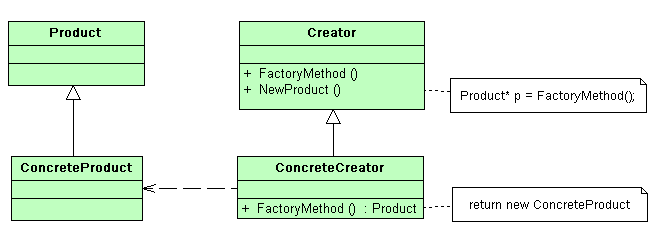
\includegraphics[width=0.9\linewidth]{architech}}
\caption{Основной алгоритм}
\label{architech:architech}
\end{figure}

Использование данного шаблона позволило нам разбить наш проект на независимые модули, что весьма упростило задачу разработки, так как написание алгоритма для конкретного таска не влияло на остальную часть проекта. При разработке был реализован базовый класс для работы с образом диска. Данный клас предназначался для формирования списка настроек, определения операционной системы на смонтированном образе и инстанционировании и накапливание всех необходимых классов-тасков в очереди тасков. После чего каждый таск из очереди отправлялся на выполнение. Блоксхема работы алгоритма (тут картинка alg_main.eps)

Каждый класс-таск порождался путем наследования от базового абстрактного класса который имеет 8 методов и 3 атрибута:

\begin{enumerate}
\item QString manual() - возвращает справку о входных параметрах данного таска;
\item void setOption(QStringList list) - установка флагов для поданных на вход параметров;
\item QString command() - возвращает команду для инициализации такска вручную;
\item bool supportOS(const coex::typeOS \&os) - возвращает флаг, указывающий на возможность использования данного таска для конкретной операционной системы;
\item QString name() - возвращает имя данного таска;
\item QString description() - возвращает краткое описание таска;
\item bool test() - предназначена для теста на доступность таска;
\item bool execute(const coex::config \&config) - запуск таска на выполнение;
\item QString m\_strName - хранит имя таска;
\item QString m\_strDescription - хранит описание таска;
\item bool m\_bDebug - флаг для параметра --debug;
\end{enumerate}

На данный момент в проекте используется восемь классов. UML-диаграмма классов представлена на рисунке (тут картинка UML.eps)

Классы taskSearchSyslogsWin, taskSearchPidginWin и taskSearchSkypeWin - наследники от класса task являются тасками. Класс winEventLog и _EVENTLOGRECORD предназначины для конвертации журнальных файлов операционной системы Windows XP, а класс writerMessages для преобразования истории переписки.

 % --------Отчет Макса---------------%
\newpage
\subsection{Плагин TaskViber}
\subsubsection{Расположения файлов мессенджера Viber}
 
В зависимости от операционной системы (в дальнейшем ОС) у Viber разные пути установки. Для Windows XP: C:\textbackslash Documents and Settings\textbackslash \%Username\%\textbackslash Application Data\textbackslash ViberPC.
Для Windows 7, 8, 8.1, 10: C:\textbackslash Users\textbackslash \%Username\%\textbackslash AppData\textbackslash Roaming\textbackslash ViberPC (рис.~\ref{kucher_1:kucher_1}).
 
\begin{figure}[h!]
\center{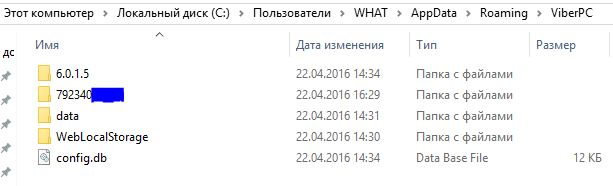
\includegraphics[width=0.8\linewidth]{kucher_1}}
\caption{ Путь к файлам Viber }
\label{kucher_1:kucher_1}
\end{figure}

\subsubsection{Описание содержимого папки «ViberPC»}

При изучении содержимого папки «ViberPC» было обнаружено, что интересующая информация содержится в папках, название которых – номер телефона (рис.~\ref{kucher_2:kucher_2}).
	

\begin{figure}[h!]
\center{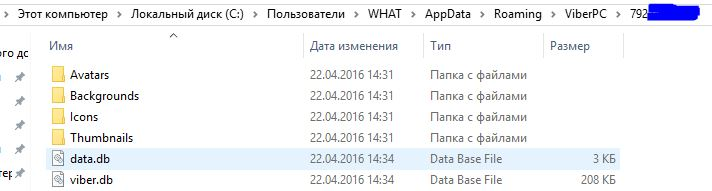
\includegraphics[width=0.8\linewidth]{kucher_2}}
\caption{ Содержимое папки с номером телефона }
\label{kucher_2:kucher_2}
\end{figure} 

\begin{itemize}
  \item Папка «Avatars» – содержит изображения пользователей;
  \item Папка «Thumbnails» – содержит все изображения, которые были отправлены и получены в ходе переписки;
	«viber.db» – база данных (далее БД), в которой хранится информация о контактах, переписках, звонках.
	БД «viber.db» – имеет формат SQLite format 3 (рис.~\ref{kucher_3:kucher_3}).
\end{itemize}
 
\begin{figure}[h!]
\center{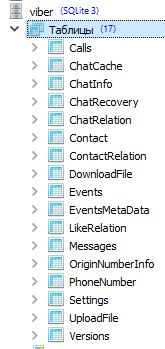
\includegraphics[width=0.3\linewidth]{kucher_3}}
\caption{ Содержимое БД «viber.db» }
\label{kucher_3:kucher_3}
\end{figure} 

\subsubsection{SQL-запросы для получения информации}

Чтобы получить все контакты и их имена был написан следующий SQL-запрос: 
\textit{Select ContactRelation.Number, Contact.FirstName from СontactRelation, Contact where Contact.ContactID = ContactRelation.ContactID}.

Чтобы получить все контакты и имена, на которые можно позвонить в Viber, нужен следующий SQL-запрос: 
\textit{Select Contact.FirstName, ContactRelation.Number from contact, PhoneNumber, ContactRelation where PhoneNumber.IsViberNumber = 1 and PhoneNumber.Number = ContactRelation.Number and ContactRelation.ContactID = Contact.ContactID}.

Чтобы связать изображение пользователя с номером телефона и именем, нужен следующий SQL-запрос:
\textit{Select Contact.FirstName, ContactRelation.Number, OriginNumberInfo.AvatarPath From OriginNumberInfo, ContactRelation, Contact Where OriginNumberInfo.Number = ContactRelation.Number and ContactRelation.ContactID = Contact.ContactID}.

Для получения информации о звонках которые осуществлялись через Viber, нужен следующий запрос: 
\textit{select Contact.FirstName, Events.Direction, datetime(Events.TimeStamp, 'unixepoch') from Contact, Events, ContactRelation where Events.EventID = (select Calls.EventID from Calls) AND Events.Number = ContactRelation.Number and ContactRelation.ContactID = Contact.ContactID}.

Для получения текста переписки с конкретным пользователем нужно знать его номер чата. Для получения всех номеров чата нужно воспользоваться следующим запросом: 
\textit{Select ChatInfo.ChatID, Contact.FirstName, ChatInfo.TokenFrom ChatInfo, ContactRelation, Contactwhere ChatInfo.Token = ContactRelation.Number and ContactRelation.ContactID = Contact.ContactID}.

Зная номер чата, можно получить текст переписки: 
\textit{select Messages.Body, Contact.FirstName, Events.Direction, Messages.ThumbnailPath, datetime(Events.TimeStamp, 'unixepoch') from messages, Events, Contact, ContactRelation where Messages.EventID = Events.EventID and Events.Number = ContactRelation.Number and ContactRelation.ContactID = Contact.ContactID and Events.ChatID = @nomer\_chata}.

\subsubsection{Описание плагина}

Плагин «TaskViber» получает точку монтирования жесткого диска, с которого, в отличии от ОС, проверяет папку «ViberPC» у всех пользователей в ОС. Если папка «ViberPC» существует, то плагин извлекает информацию из аккаунтов, под которыми авторизовались с данного компьютера. Всю найденную информацию плагин сохраняет по указанному пути программного обеспечения «COEX». В папку «Avatars» (рис.~\ref{kucher_9:kucher_9}) копируются все найденные изображения пользователей. В папку «Thumbnails» (рис.~\ref{kucher_10:kucher_10}) копируются все изображения, которые были отправлены и получены в ходе переписки. В файле «Avatar Path.txt» находятся связи между изображениями пользователей, именами и номерами телефонов. В файле «Calls.txt» находятся описание звонков, которые осуществлялись через «Viber» (с кем был звонок, во сколько и кто кому звонил). В файле «Phone book.txt» находятся все номера телефонов и имена с мобильного телефона, на котором был зарегистрирован аккаунт в «Viber». В файле «Viber book.txt» находятся все номера телефонов и имена, которым можно позвонить через «Viber». В файле «Имя/номер messages.txt» содержится переписка с пользователем «Имя/номер» (с кем велась переписка, кто кому писал, что писал и во сколько писал).

Алгоритм работы плагина «TaskViber» представлен на рисунке~\ref{kucher_4:kucher_4}, алгоритм функции WinXP --- на рисунке~\ref{kucher_5:kucher_5}. Ниже также представлены алгоритмы работы Win\_7\_8\_10 (рис.~\ref{kucher_6:kucher_6}) и Viber\_XP\_7\_8\_10 (рис.~\ref{kucher_7:kucher_7}).

Результат работы плагина представлен на рисунке~\ref{kucher_8:kucher_8}.
 

\begin{figure}[h!]
\center{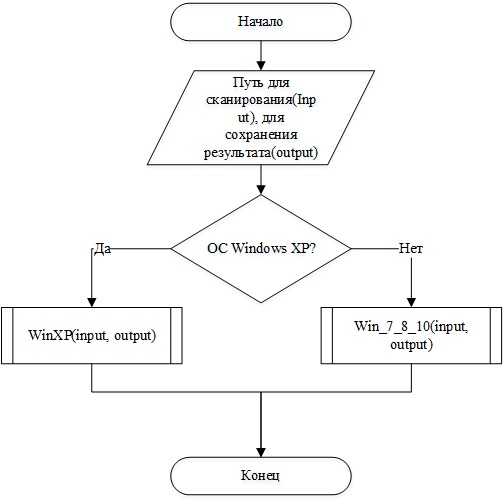
\includegraphics[width=0.6\linewidth]{kucher_4}}
\caption{ Алгоритм работы плагина }
\label{kucher_4:kucher_4}
\end{figure} 
  
\begin{figure}[h!]
\center{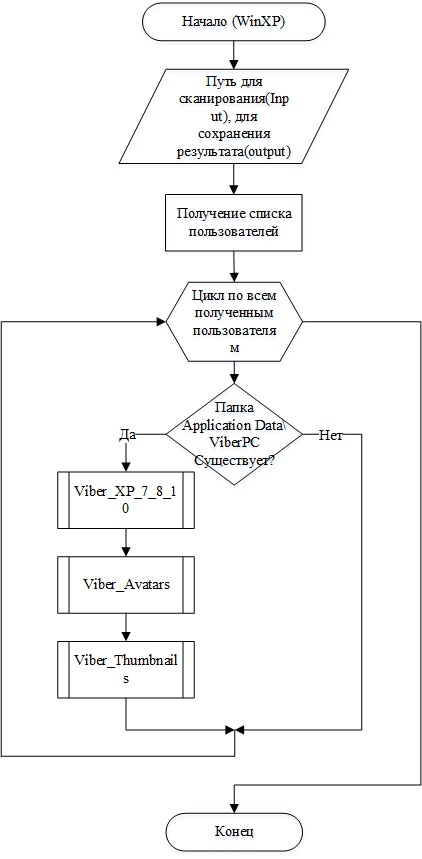
\includegraphics[width=0.6\linewidth]{kucher_5}}
\caption{ Алгоритм работы функции WinXP }
\label{kucher_5:kucher_5}
\end{figure} 

\begin{figure}[ht]
\center{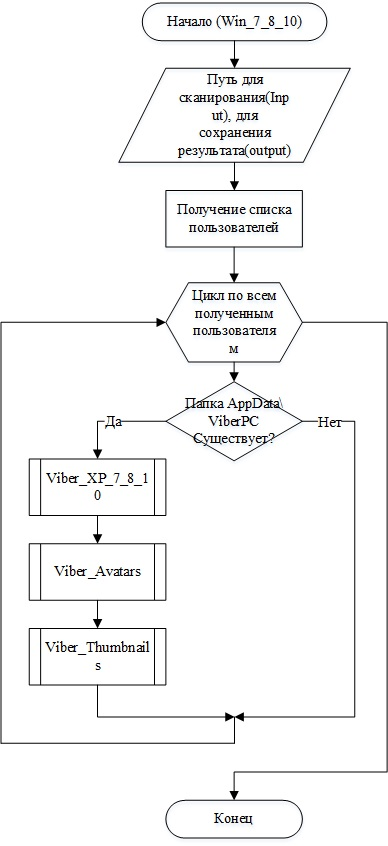
\includegraphics[width=0.6\linewidth]{kucher_6}}
\caption{ Алгоритм работы Win\_7\_8\_10 }
\label{kucher_6:kucher_6}
\end{figure} 

\begin{figure}[h!]
\center{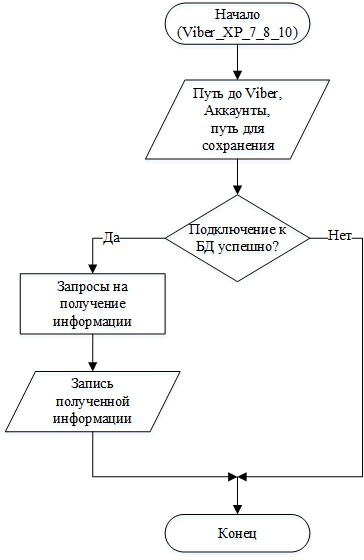
\includegraphics[width=0.5\linewidth]{kucher_7}}
\caption{ Алгоритм работы Viber\_XP\_7\_8\_10 }
\label{kucher_7:kucher_7}
\end{figure} 

\clearpage

\begin{figure}[h!]
\center{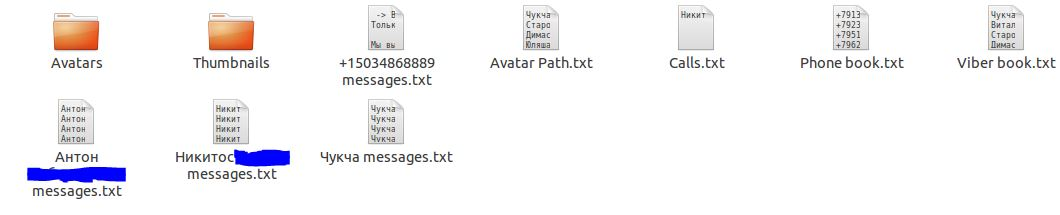
\includegraphics[width=1\linewidth]{kucher_8}}
\caption{ Результат работы плагина }
\label{kucher_8:kucher_8}
\end{figure} 

\begin{figure}[h!]
\center{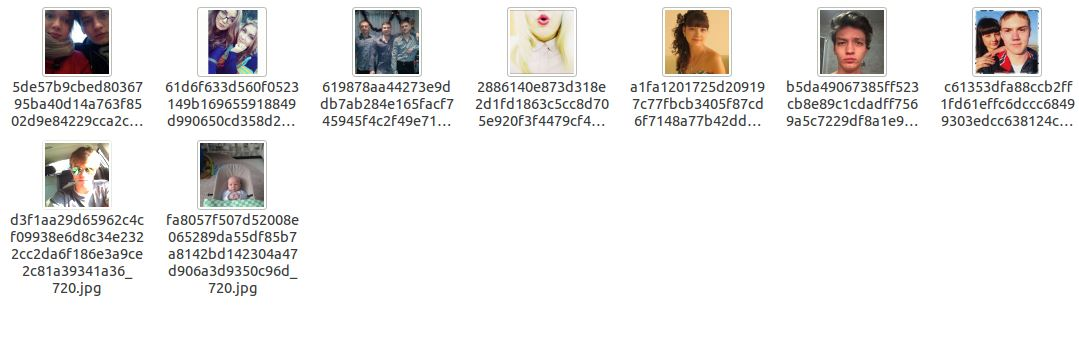
\includegraphics[width=1\linewidth]{kucher_9}}
\caption{ Содержимое папки «Avatars» }
\label{kucher_9:kucher_9}
\end{figure} 

\begin{figure}[h!]
\center{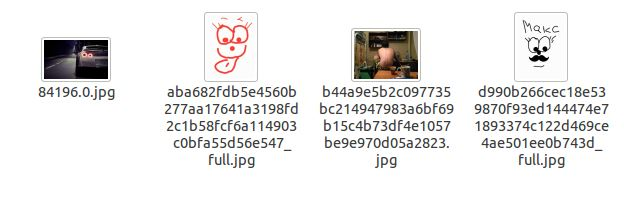
\includegraphics[width=0.8\linewidth]{kucher_10}}
\caption{ Содержимое папки «Thumbnails» }
\label{kucher_10:kucher_10}
\end{figure} 

\clearpage


 % ---------Отчет Юры----------------%
\newpage
\subsection{Сбор сохраненных логинов и паролей браузера Mozilla Firefox}
Главной задачей в данном стало написание программного модуля для сбора сохраненных логинов и паролей браузера Mozilla Firefox.

Сохраненные логины и пароли хранятся в папке с профилем Mozilla Firefox. Путь к папке: C:\textbackslash Users\textbackslash User\textbackslash AppData\textbackslash Roaming\textbackslash Mozilla\textbackslash Firefox\textbackslash Profiles\textbackslash prof\_n. Где prof\_n генерируется самим браузером.

Для браузеров, версия которых 31 и меньше, логины и пароли хранятся в файле базы данных signons.sqlite. База данных имеет формат sqlite3. В базе данных есть таблица moz\_logins. В ней нас интересуют столбцы: encryptedUsername, encryptedPassword, formSubmitURL, которые содержат зашифрованный логин, зашифрованный пароль и URL сайта соответственно.

Для остальных, логины и пароли хранятся в файле logins.json.

Json – текстовый формат файла, в котором информация представлена в виде структур. На рисунке~\ref{teresh_1:teresh_1} показано, как выглядит файл logins.json.

\begin{figure}[h!]
\center{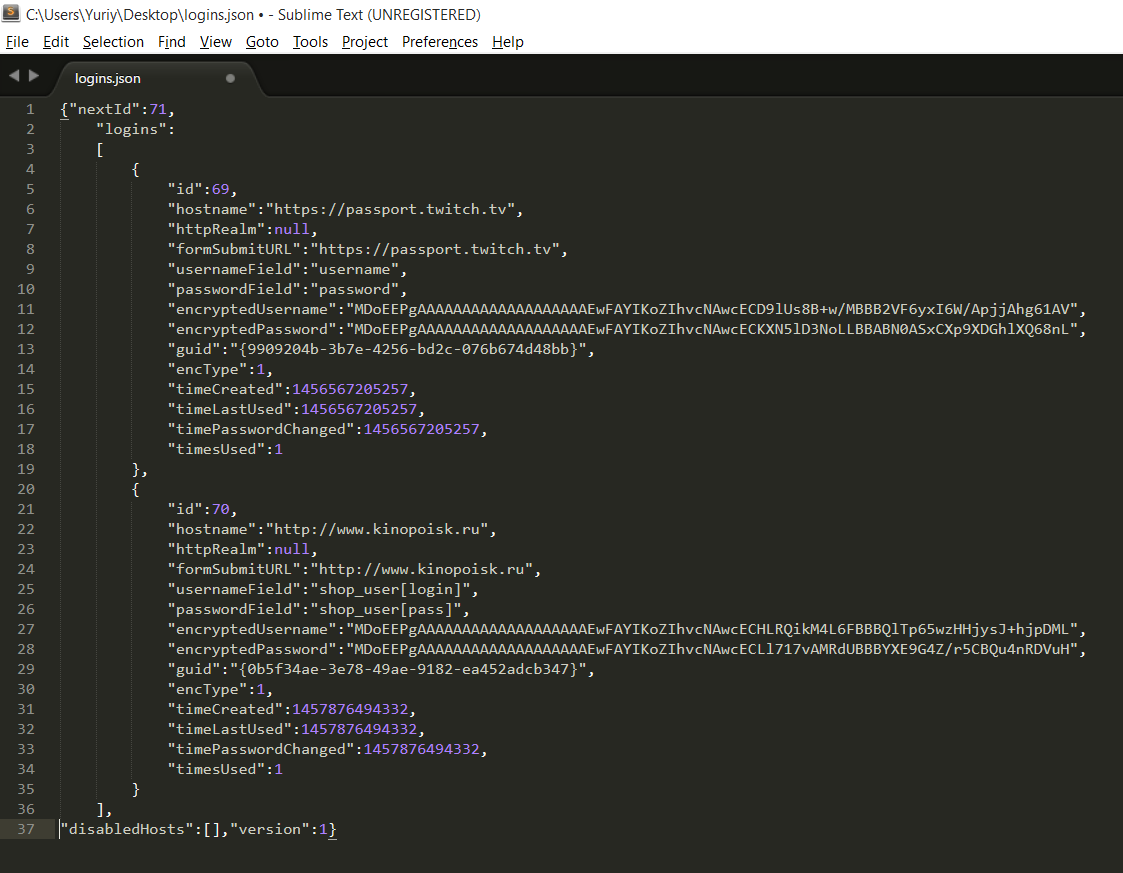
\includegraphics[width=0.9\linewidth]{teresh_1}}
\caption{Файл logins.json}
\label{teresh_1:teresh_1}
\end{figure}

Здесь нас интересуют те же самые поля, как и в случае с базой данных.

Как видно из рисунка~\ref{teresh_1:teresh_1}, логины и пароли зашифрованы. Для их расшифровки нам также необходимы файлы cert8.db, key3.db и secmod.db. В них содержатся ключи для расшифровки значений. Эти файлы также находятся в папке с профилем.

Так же для работы модуля необходима библиотека nss3. Именно с помощью нее браузер зашифровывает логины и пароли.

Nss3 – open source библиотека, разработанная для создания кроссплатформенных защищенных клиентских и серверных приложений.

\subsubsection{Алгоритм работы программного модуля}

Сначала модуль подключает стороннюю библиотеку nss3. Затем выполняется поиск файла compatibility.ini (также находится в папке профиля), содержащего версию браузера.

Для браузеров, версия которых 31 и меньше, ищется файл базы данных signons.sqlite. Модуль подключается к нему и выполняет sql-запрос: «SELECT encryptedUsername, encryptedPassword, formSubmitURL FROM moz\_logins».

Для других версий, ищется файл logins.json, вытаскиваются нужные нам значения.

Затем данные расшифровываются с помощью сторонней библиотеки nss3 и сохраняются в xml-файл.

Блок-схема алгоритма работы программы представлена на рисунке~\ref{teresh_2:teresh_2}.

\begin{figure}[h!]
\center{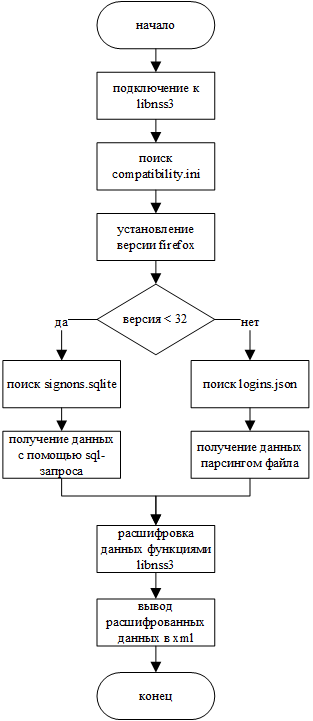
\includegraphics[width=0.6\linewidth]{teresh_2}}
\caption{Алгоритм работы программного модуля}
\label{teresh_2:teresh_2}
\end{figure}

\subsubsection{Тестирование}

Как видно из рисунков~\ref{teresh_3:teresh_3} и~\ref{teresh_4:teresh_4} плагин выполняет поставленные перед ним задачи.

\begin{figure}[h!]
\center{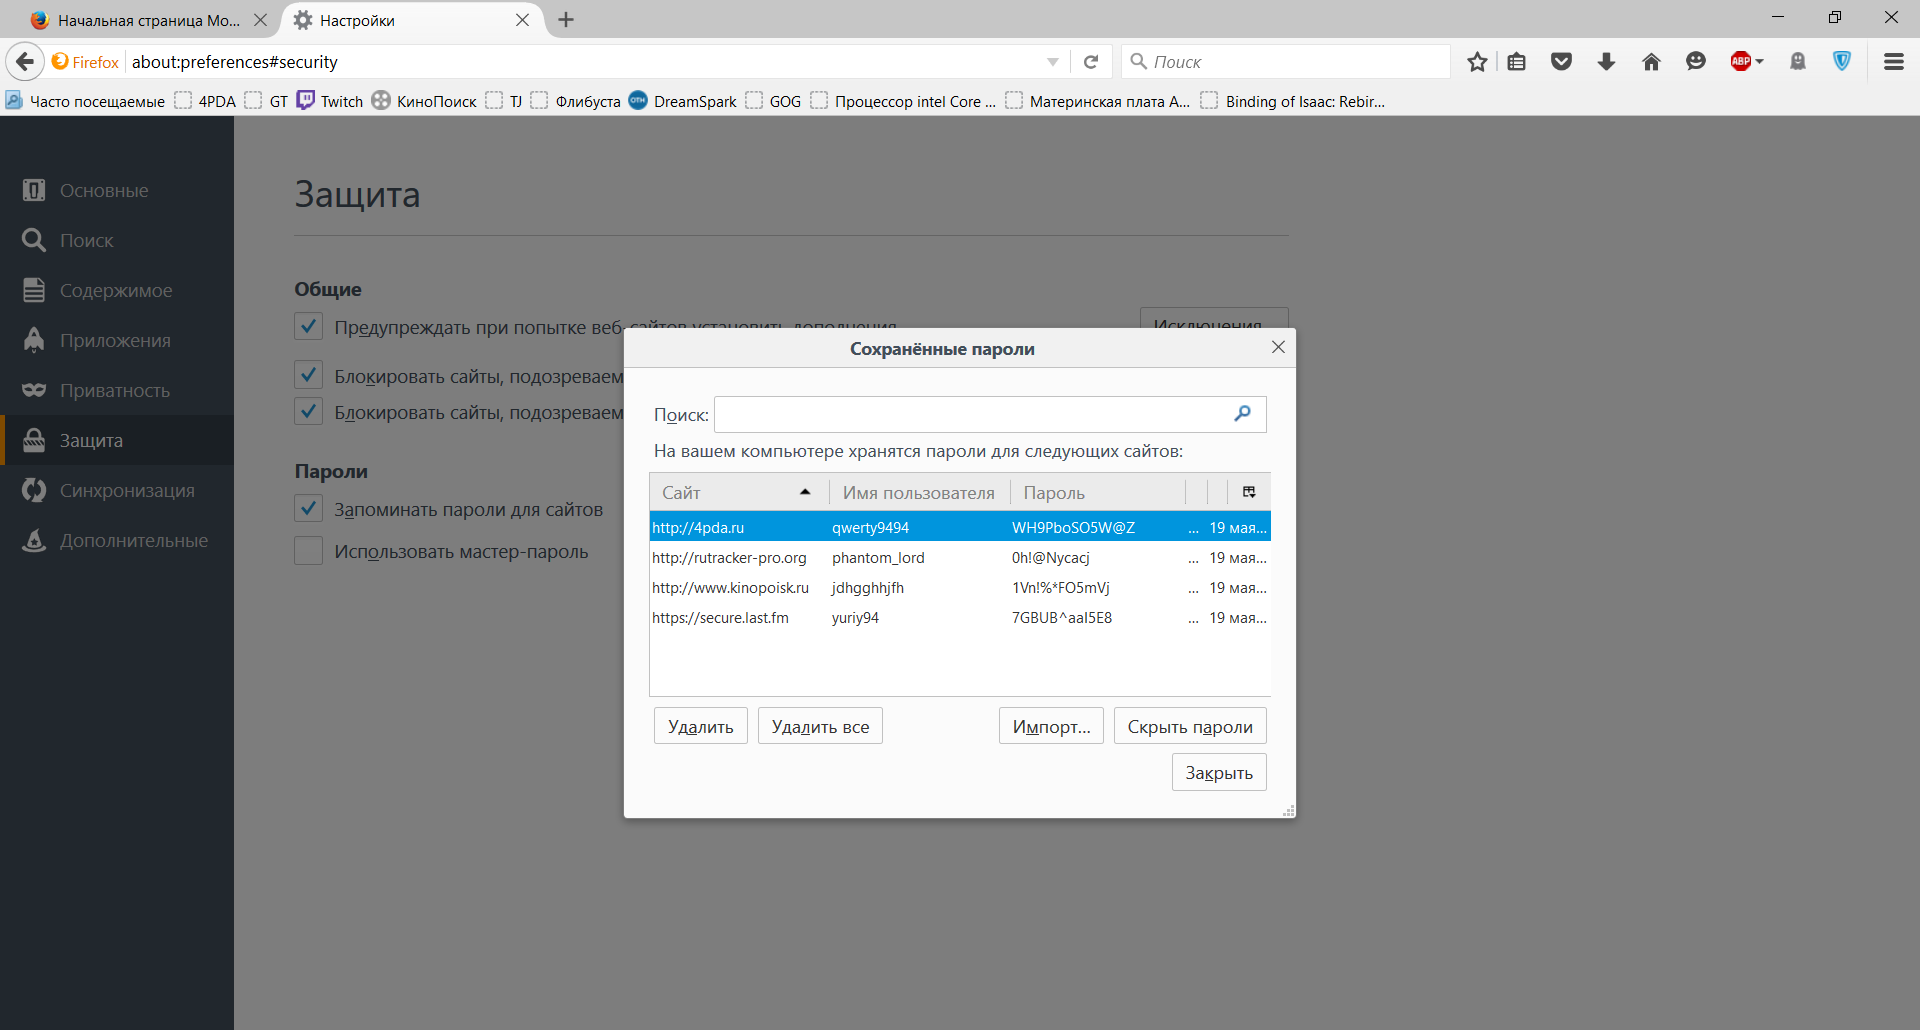
\includegraphics[width=0.9\linewidth]{teresh_3}}
\caption{Тестовые данные}
\label{teresh_3:teresh_3}
\end{figure}

\begin{figure}[h!]
\center{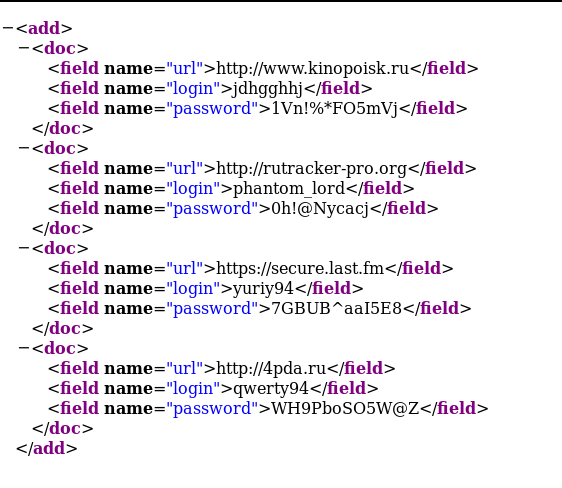
\includegraphics[width=0.9\linewidth]{teresh_4}}
\caption{Результат тестирования}
\label{teresh_4:teresh_4}
\end{figure}

\clearpage



 % ---------Отчет Влада--------------%
\newpage
\subsection{Графический интерфейс пользователя системы <<COEX>>}


\begin{figure}[h!]
\center{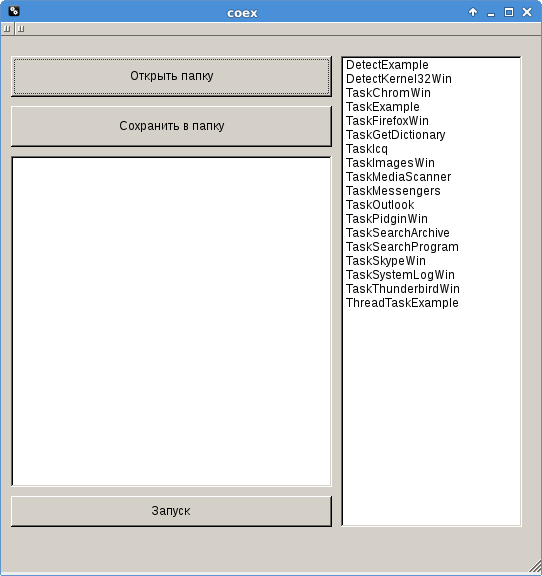
\includegraphics[width=0.7\linewidth]{ship_1}}
\caption{ Предыдущая версия интерфейса }
\label{ship_1:ship_1}
\end{figure}

\begin{figure}[h!]
\center{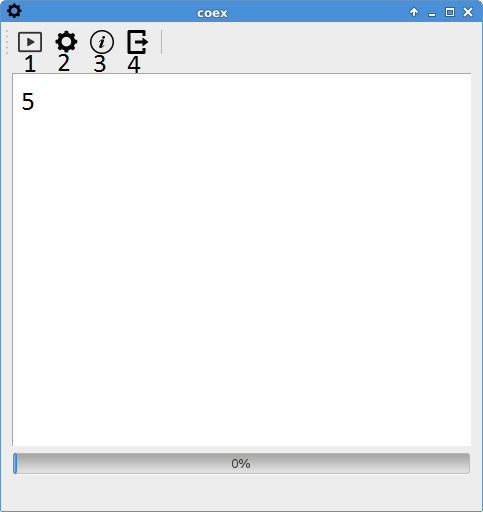
\includegraphics[width=0.7\linewidth]{ship_2}}
\caption{ Главное окно нового интерфейса }
\label{ship_2:ship_2}
\end{figure}

Новый интерфейс состоит из следующих элементов:
\begin{enumerate}
  \item элемент отвечающий за запуск coex;
  \item элемент отвечающий за настройки;
  \item сведения о программе;
  \item кнопка закрытия приложения;
  \item область вывода промежуточной информации.
\end{enumerate}

\begin{figure}[h!]
\center{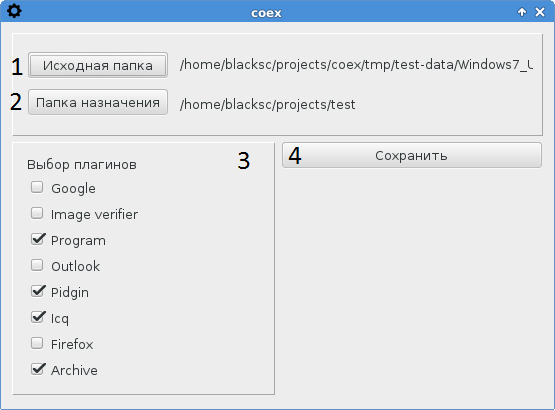
\includegraphics[width=0.7\linewidth]{ship_3}}
\caption{ Окно настроек }
\label{ship_3:ship_3}
\end{figure}

Интерфейс окна настроек состоит из следующих элементов:
\begin{enumerate}
  \item элемент <<исходная папка>> отвечает выбор папки, в которой будет производиться поиск;
  \item элемент <<папка назначения>> отвечает за выбор папки для сохранения результатов;
  \item данная область отвечает за выбор компонентов coex;
  \item элемент <<Сохранить>> отвечает за сохранения выбранных настроек.
\end{enumerate}

При следующем запуске приложения будут загружены сохраненные раннее настройки, а также геометрия главного приложения и его состояние т.е. оно откроется в том месте где его закрыли. Также данное окно является модальным т.е. оно прерывают работу главного окна и для продолжения его работы такое окно должно быть закрыто.

Для простоты предполагается, что организация называется TUSUR, а приложение называется coex данные параметры прописываются в исходном коде приложения. Настройки будут храниться по-разному в зависимости от платформы.

  В системах Unix:
\begin{enumerate}
  \item HOME/.config/TUSUR/coex.conf;
  \item HOME/.config/coex.conf;
  \item /etc/xdg/TUSUR/coex.conf;
  \item /etc/xdg/TUSUR/.conf.
\end{enumerate}

  В Mac OS
\begin{enumerate}
  \item HOME/Library/Preferences/com.TUSUR.coex.plist;
  \item HOME/Library/Preferences/com.TUSUR.plist;
  \item /Library/Preferences/com.TUSUR.coex.plist;
  \item /Library/Preferences/com.TUSUR.plist.
\end{enumerate}

  В Windows настройки хранятся по следующим путям реестра:
\begin{enumerate}
  \item HKEY\_CURRENT\_USER\textbackslash Software\textbackslash TUSUR\textbackslash coex;
  \item <<HKEY\_CURRENT\_USER\textbackslash Software\textbackslash TUSUR>>;
  \item <<HKEY\_LOCAL\_MACHINE\textbackslash Software\textbackslash TUSUR\textbackslash coex>>;
  \item <<HKEY\_LOCAL\_MACHINE\textbackslash Software\textbackslash TUSUR>>.
\end{enumerate}
  

Содержание файла настроек представлено на рисунке~\ref{ship_25:ship_25}.

\begin{figure}[h!]
\center{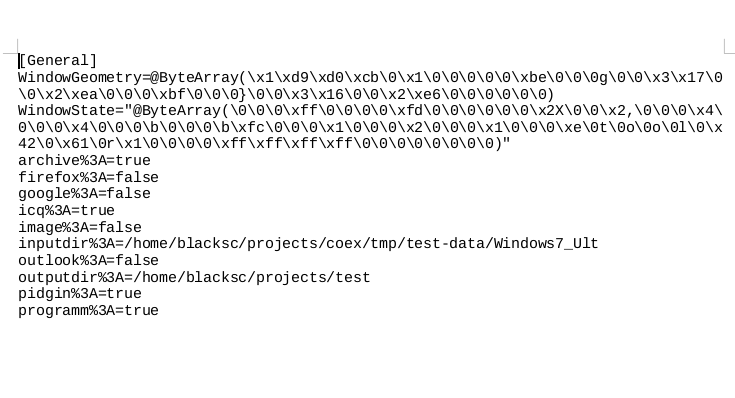
\includegraphics[width=0.9\linewidth]{ship_25}}
\caption{ Содержание файла настроек }
\label{ship_25:ship_25}
\end{figure}  

\begin{figure}[h!]
\center{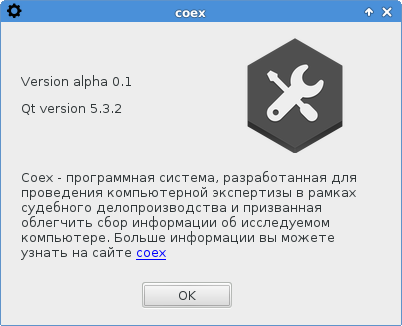
\includegraphics[width=0.7\linewidth]{ship_4}}
\caption{ О программе }
\label{ship_4:ship_4}
\end{figure}

\begin{figure}[h!]
\center{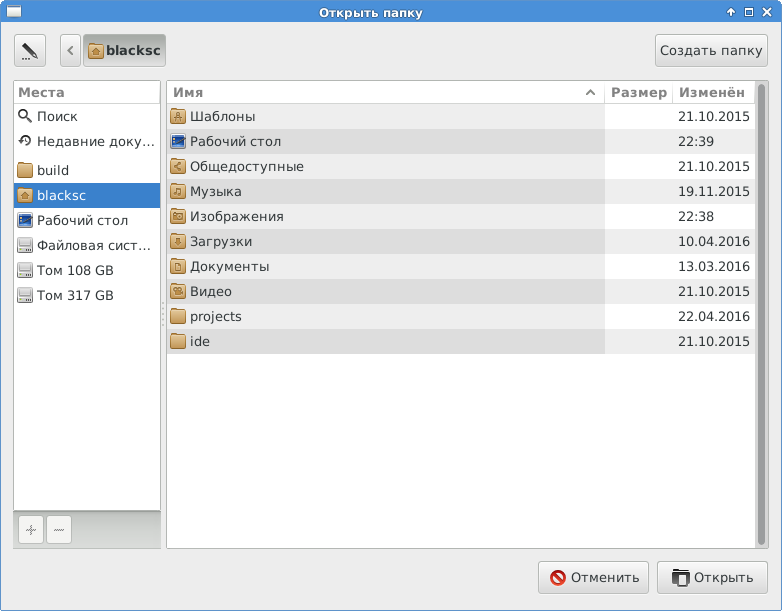
\includegraphics[width=0.7\linewidth]{ship_5}}
\caption{ Выбор директорий }
\label{ship_5:ship_5}
\end{figure}

Если не выбраны директории для работы, то при нажатии на кнопку “Запуск” отобразиться соответствующее сообщение (рисунок ~\ref{ship_6:ship_6}). Диалоговое окно выбора директории представлено на рисунке ~\ref{ship_5:ship_5}. По завершению работы системы отобразиться соответствующие сообщение (рисунок ~\ref{ship_7:ship_7}), при этом если нажать на кнопку “Результаты”, то откроется директория с результатами работы (рисунок ~\ref{ship_8:ship_8}).

\begin{figure}[h!]
\center{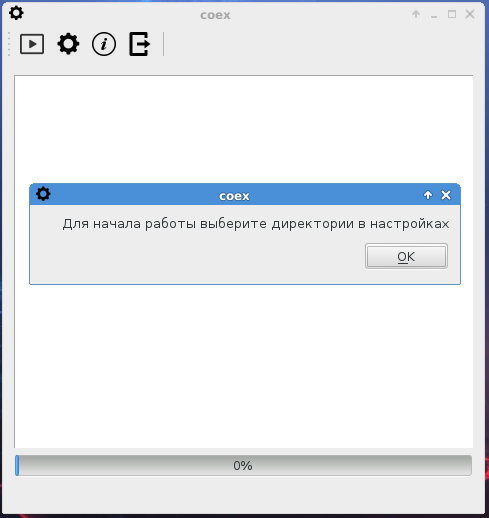
\includegraphics[width=0.7\linewidth]{ship_6}}
\caption{ Сообщение об ошибке }
\label{ship_6:ship_6}
\end{figure}

\begin{figure}[h!]
\center{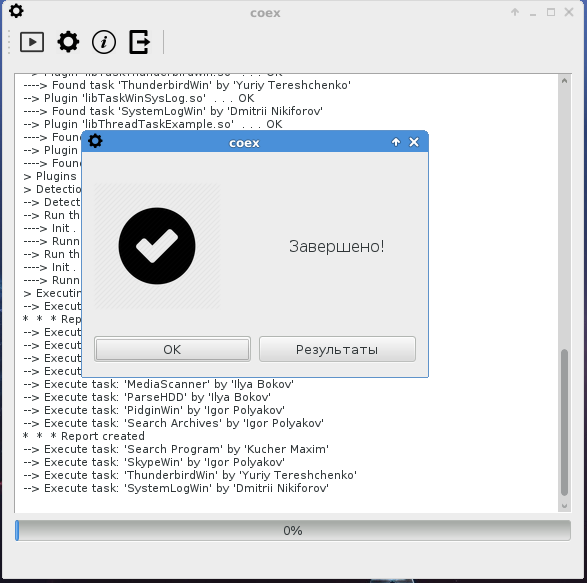
\includegraphics[width=0.7\linewidth]{ship_7}}
\caption{ Завершение работы }
\label{ship_7:ship_7}
\end{figure}

\begin{figure}[h!]
\center{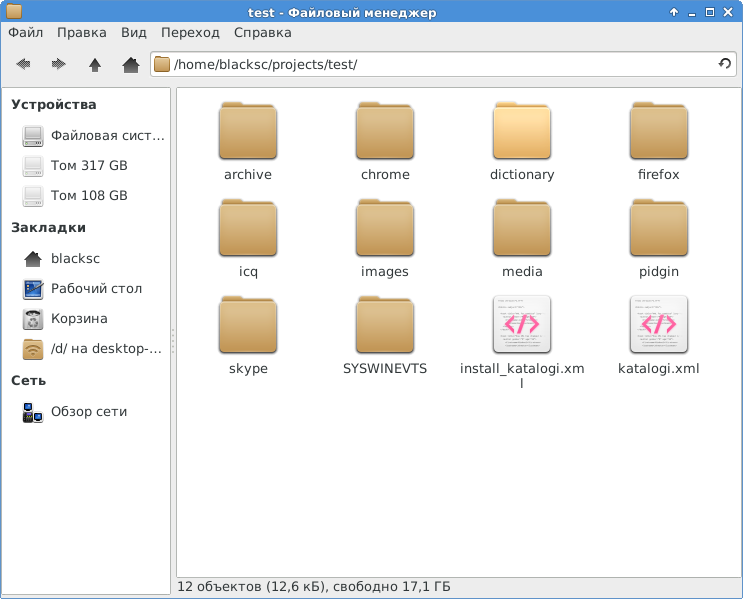
\includegraphics[width=0.7\linewidth]{ship_8}}
\caption{ Папка с результатами }
\label{ship_8:ship_8}
\end{figure}

\clearpage

\newpage
\subsection{Анализ данных с помощью Apache Solr}
\subsubsection{Общая информация об Apache Lucene, Solr}

Apache Solr - это расширяемая поисковая платформа от Apache. Система основана на библиотеке Apache Lucene и разработана на Java. Особенности ее в том, что она представляет из себя не просто техническое решение для поиска, а именно платформу, поведение которой можно легко расширять/менять/настраивать под любые нужды - от обычного полнотекстового поиска на сайте до распределенной системы хранения/получения/аналитики текстовых и других данных с мощным языком запросов. Lucene — самый известный из поисковых движков, изначально ориентированный именно на встраивание в другие программы.

\subsubsection{Подготовка окружения и установка Apache Lucene}
Добавление репозитория:
\textit
{
deb http://ppa.launchpad.net/webupd8team/java/ubuntu trusty main
deb-src http://ppa.launchpad.net/webupd8team/java/ubuntu trusty main
} (рис.~\ref{ship_9:ship_9}).

\begin{figure}[h!]
\center{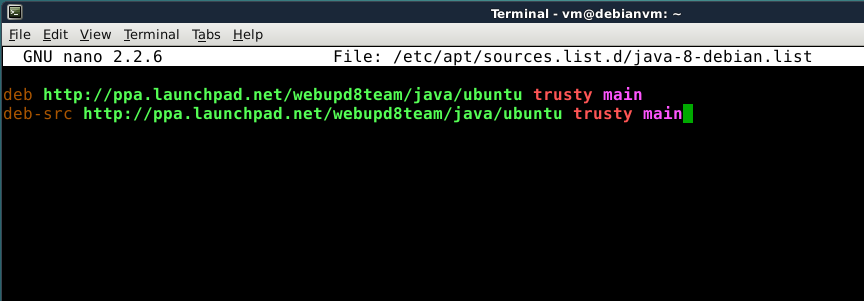
\includegraphics[width=1\linewidth]{ship_9}}
\caption{Добавление репозитория}
\label{ship_9:ship_9}
\end{figure}

Добавления ключа репозитория:
  \textit{
apt-key adv --keyserver hkp://keyserver.ubuntu.com:80 --recv-keys EEA14886
} (рис.~\ref{ship_10:ship_10}).

\begin{figure}[h!]
\center{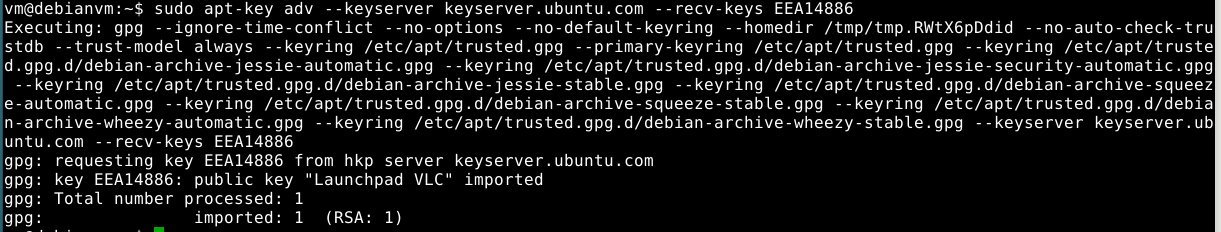
\includegraphics[width=1\linewidth]{ship_10}}
\caption{Добавление ключа}
\label{ship_10:ship_10}
\end{figure}

Обновление списка пакетов:
\textit
{
apt-get update
} (рис.~\ref{ship_11:ship_11}).

\begin{figure}[h!]
\center{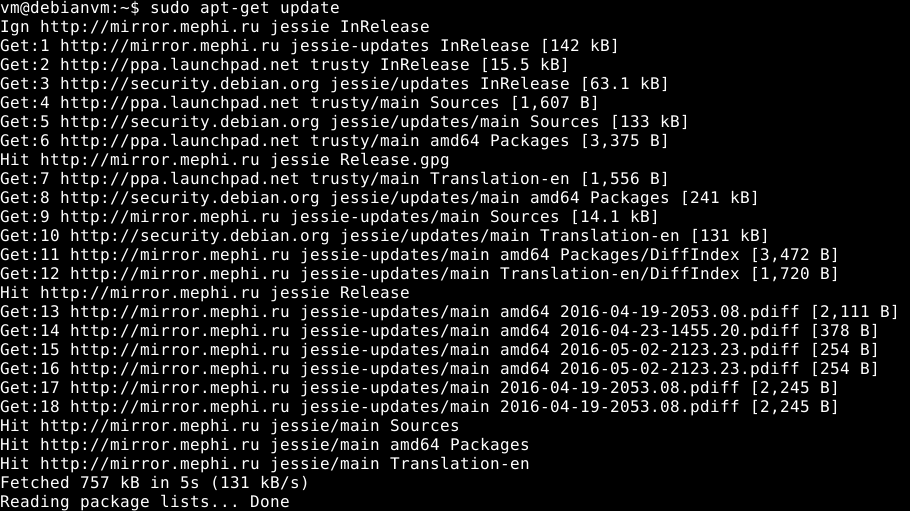
\includegraphics[width=1\linewidth]{ship_11}}
\caption{Обновление списка пакетов}
\label{ship_11:ship_11}
\end{figure}

Устанавка Java:
\textit
{
apt-get install oracle-java8-installer
} (рис.~\ref{ship_12:ship_12}).

\begin{figure}[h!]
\center{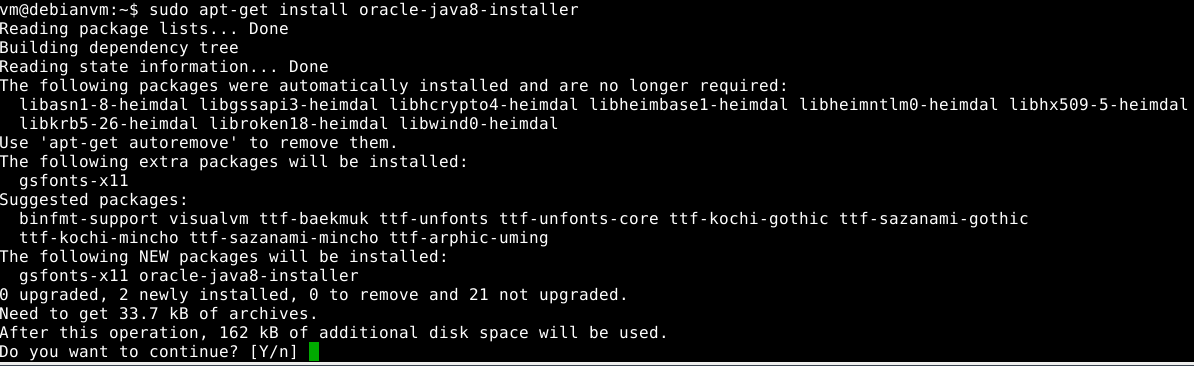
\includegraphics[width=1\linewidth]{ship_12}}
\caption{Установка java}
\label{ship_12:ship_12}
\end{figure}

Загрузка Apache Solr:
\textit
{
wget http://apache.mirror1.spango.com/lucene/solr/5.2.1/solr-5.2.1.tgz
} (рис.~\ref{ship_13:ship_13}).

\begin{figure}[h!]
\center{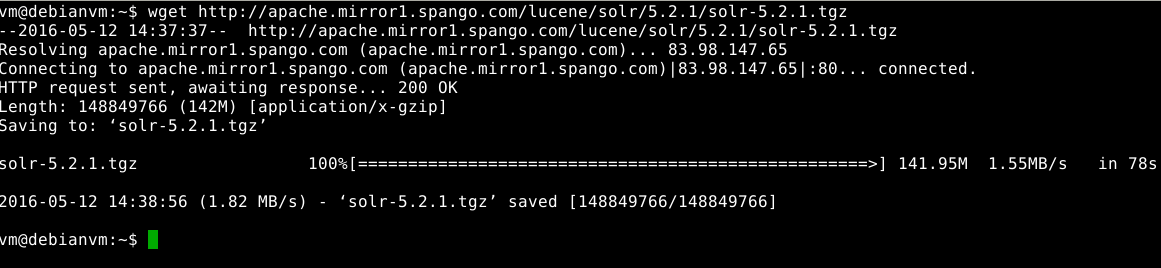
\includegraphics[width=1\linewidth]{ship_13}}
\caption{Загрузка Apache Solr}
\label{ship_13:ship_13}
\end{figure}

Распаковка архива и установка: 
\textit
{
tar xzf solr-5.2.1.tgz solr-5.2.1/bin/install\_solr\_service.sh --strip-components=2
}.
Устанавка Apache Solr командой 
\textit
{
sudo bash ./install\_solr\_service.sh solr-5.2.1.tgz
} (рис.~\ref{ship_14:ship_14}).
\begin{figure}[h!]
\center{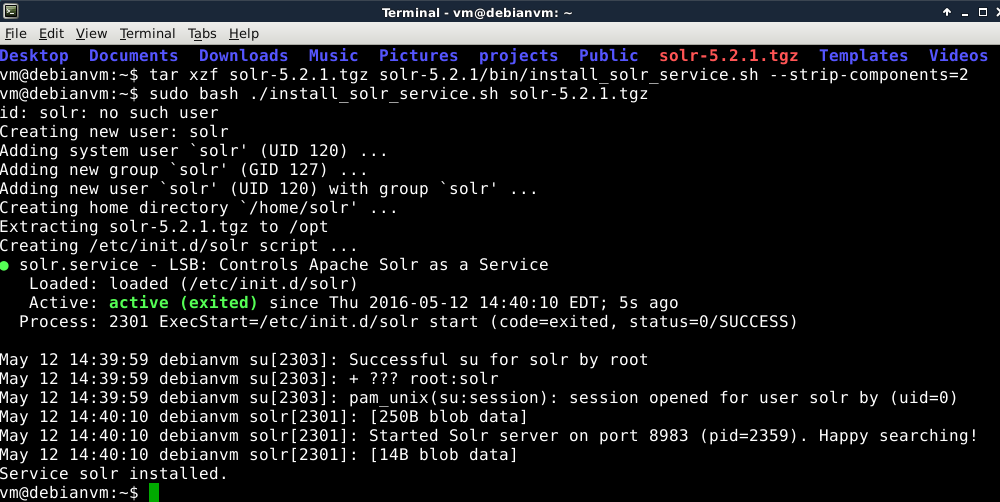
\includegraphics[width=1\linewidth]{ship_14}}
\caption{Распаковка и установка}
\label{ship_14:ship_14}
\end{figure}

Apache Solr по умолчанию работает на порту 8983. Проверка работоспособности в браузере (рис.~\ref{ship_15:ship_15}).

\begin{figure}[h!]
\center{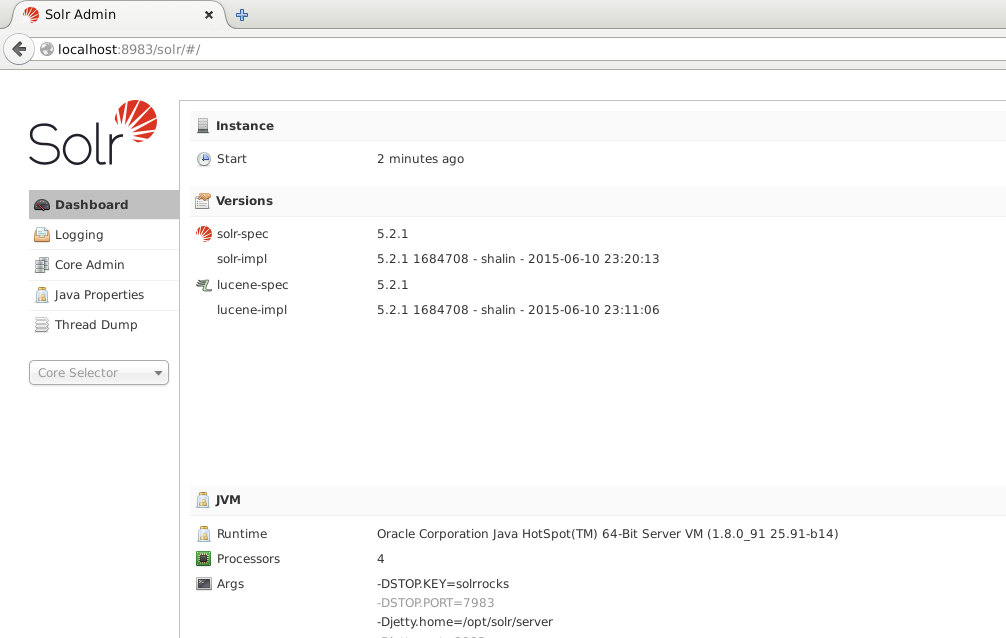
\includegraphics[width=1\linewidth]{ship_15}}
\caption{Проверка работоспособности Apache Solr}
\label{ship_15:ship_15}
\end{figure}

\subsubsection{Добавление документов в поисковый индекс}

Solr запущен, но на данный момент он не содержит каких-либо данных в поисковом индексе. 
Для отправки данных на сервер воспользуется shell скриптом, который будет брать содержимое XML файлов из необходимой директории и отправлять их Solr. В результате произошло добавления документов в Solr. Solr, в отличие от других систем хранит не документ целиком и выполняет поиск по нему, а разбивает XML-документ на поля и индексирует каждое из них  (рис.~\ref{ship_16:ship_16}).

\begin{figure}[h!]
\center{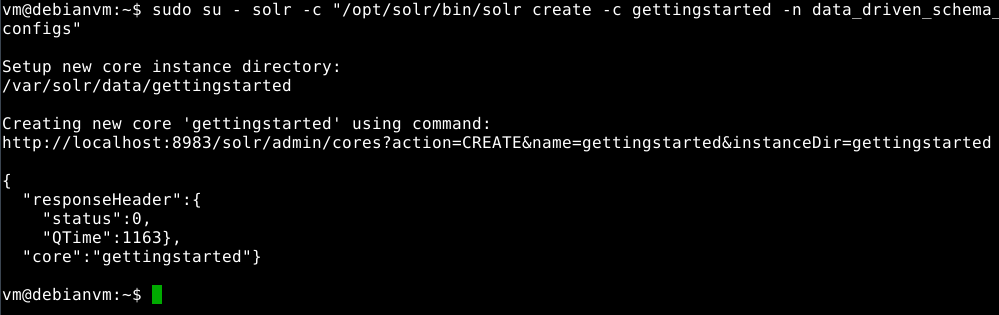
\includegraphics[width=1\linewidth]{ship_16}}
\caption{Загрузка документов}
\label{ship_16:ship_16}
\end{figure}

\subsubsection{Формирование запросов}
Так как документ в поисковом индексе представляет собой набор полей, то возможно формировать сложные поисковые запросы, которые при выполнении используют значения отдельных полей документа (рис.~\ref{ship_18:ship_18}). 

\begin{figure}[h!]
\center{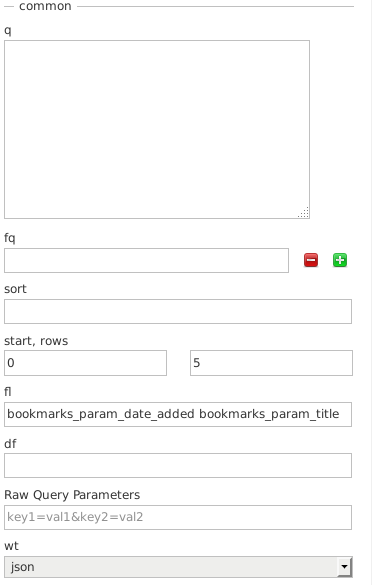
\includegraphics[width=0.4\linewidth]{ship_18}}
\caption{Область ввода запросов}
\label{ship_18:ship_18}
\end{figure}

В области для ввода запросов присутсвуют следующие поля:
\begin{enumerate}
  \item q - основной запрос;
  \item fq - фильтрующий запрос;
  \item start - сдвиг в поиске;
  \item rows - кол-во выводимых результатов;
  \item fl - выводимые поля;
  \item wt - формат вывода данных.
\end{enumerate}

Примеры запросов:
\begin{enumerate}
  \item по содержанию значения в каком-либо поле документа (рисунок ~\ref{ship_19:ship_19});
  \item по содержанию в поле определенного значения (рисунок ~\ref{ship_20:ship_20});
  \item по значению поля, находящемуся в определенном интервале (рисунок~\ref{ship_21:ship_21}, рисунок ~\ref{ship_22:ship_22}), с использованием вывода конкретных полей (рисунок~\ref{ship_23:ship_23});
  \item с использованием булевых операторов (рисунок~\ref{ship_24:ship_24}).
\end{enumerate}

\begin{figure}[h!]
\center{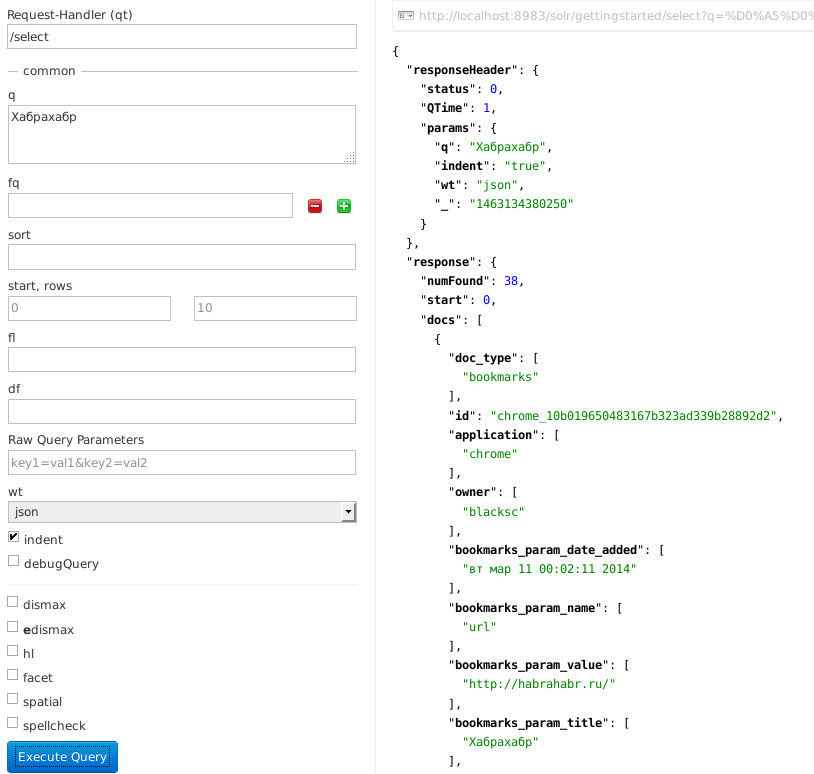
\includegraphics[width=0.7\linewidth]{ship_19}}
\caption{Запрос по содержанию в каком-либо поле документа}
\label{ship_19:ship_19}
\end{figure}

\begin{figure}[h!]
\center{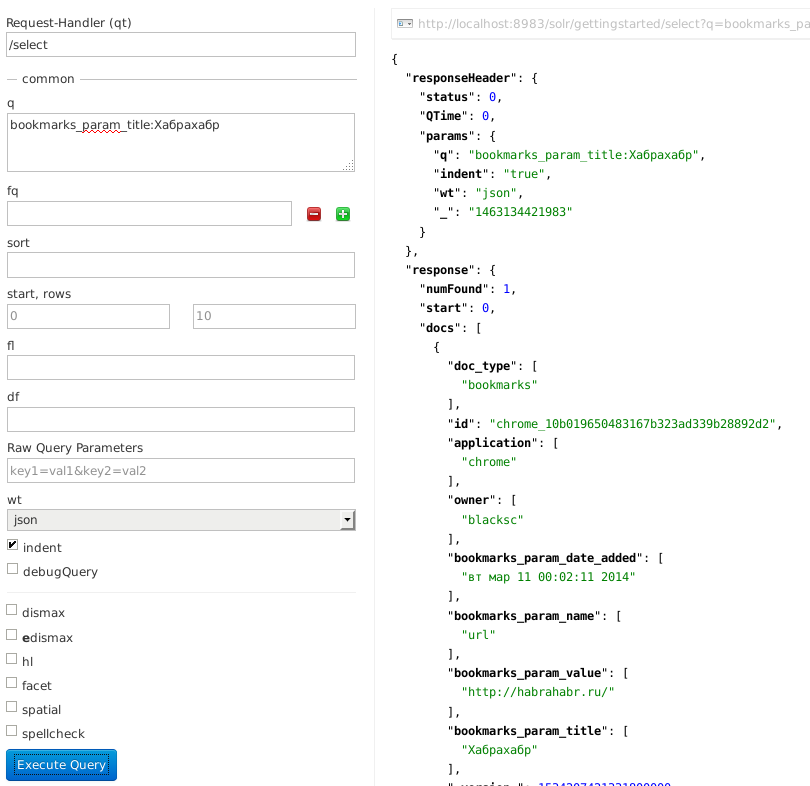
\includegraphics[width=1\linewidth]{ship_20}}
\caption{Запрос по содержанию в поле определенного значения}
\label{ship_20:ship_20}
\end{figure}

\begin{figure}[h!]
\center{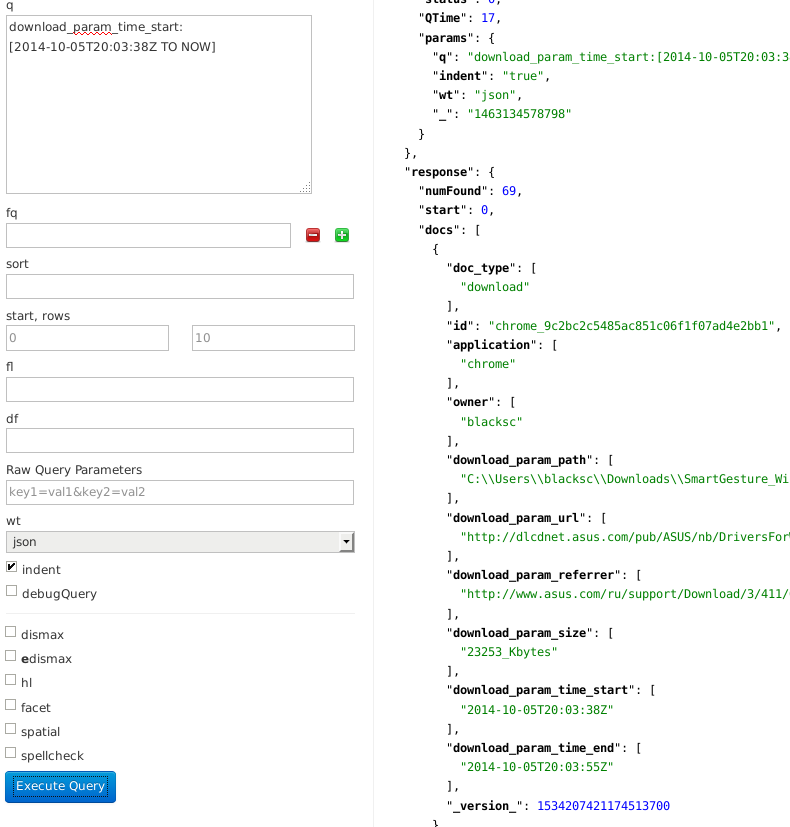
\includegraphics[width=1\linewidth]{ship_21}}
\caption{Запрос по значению поля даты, находящиеся в интервале от определенного значения до настоящего времени}
\label{ship_21:ship_21}
\end{figure}

\begin{figure}[h!]
\center{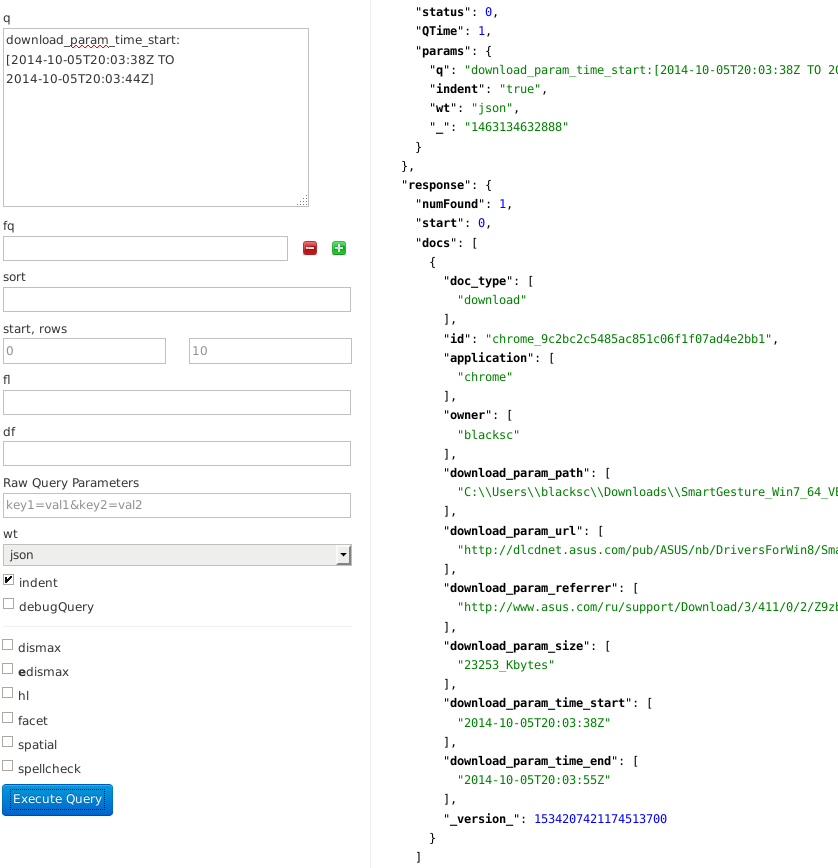
\includegraphics[width=1\linewidth]{ship_22}}
\caption{Запрос по значению поля даты, находящемуся в определенном интервале}
\label{ship_22:ship_22}
\end{figure}


\begin{figure}[h!]
\center{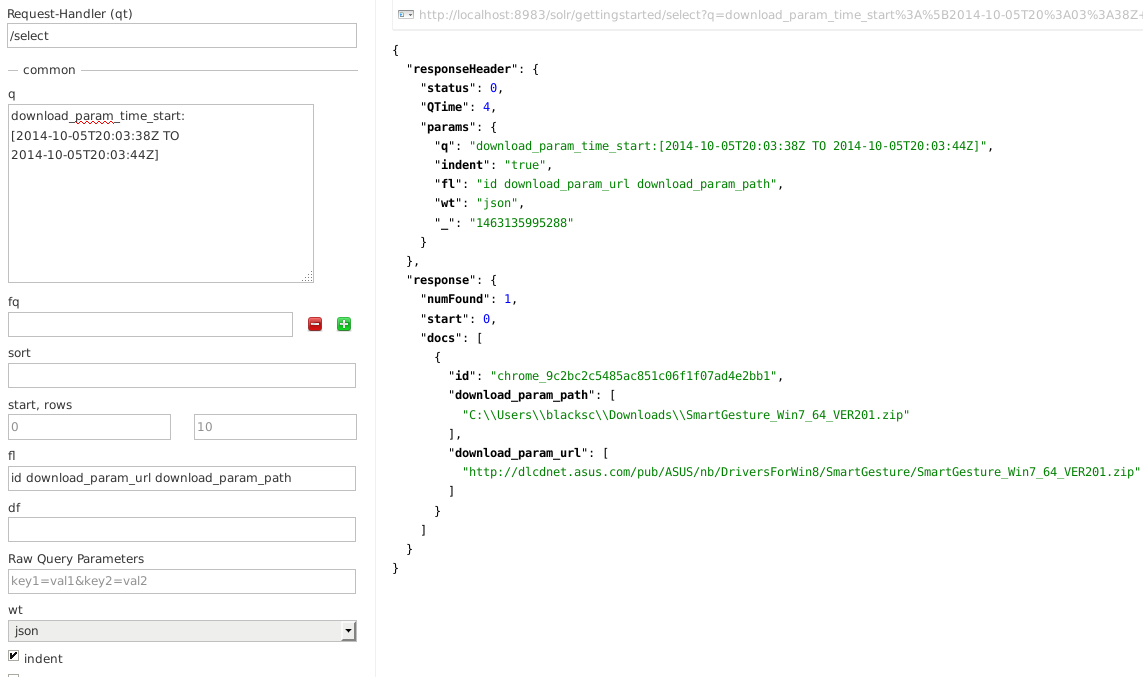
\includegraphics[width=1\linewidth]{ship_23}}
\caption{Запрос с выводом определенных полей}
\label{ship_23:ship_23}
\end{figure}

\begin{figure}[h!]
\center{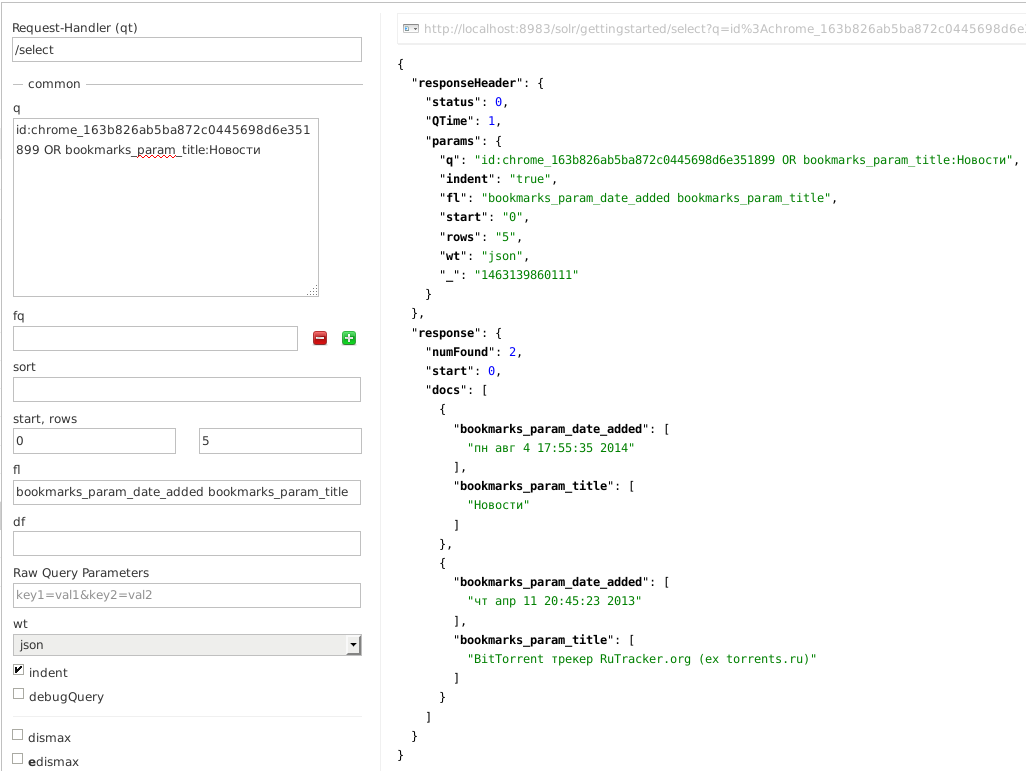
\includegraphics[width=1\linewidth]{ship_24}}
\caption{Запрос с использованием булевого оператора}
\label{ship_24:ship_24}
\end{figure}

\clearpage

 
 % ---------Отчет Андрея--------------%
\newpage
\subsection {Создание <<бинарного>> пакета .DEB из исходных файлов программного комплекса <<COEX>>} 
Для распространения и установки программного комплекса <<COEX>> на электронные вычислительные машины был выбран формат двоичного пакета *.deb. Данный пакет включает в себя все необходимые файлы для работы программы, а также содержит список зависимостей. Он имеет строго типизированную структуру и используется операционными системами Unix. Строго типизированная структура позволяет операционной системе узнавать все нужные элементы для установки и работы с данным пакетам вне зависимости от программного обеспечения (далее ПО), находящейся в данном Deb-пакете, узнавать зависимости программных библиотек, необходимых для запуска программного продукта, содержащегося в двоичном пакете.  Выбор данного формата пакета обусловлен возможностью его гибкой настройки для любого программного обеспечения (возможность использовать встроенные скрипты для настройки процесса установки ПО), поддержкой почти всеми операционными системами Unix. А также широкой распространенностью использования deb-пакетов в семействе операционных систем Unix в связи с высокой популярностью дистрибутивов операционных систем, в которой он распространяется.~\cite{tecmint}  

Для пакета *.deb содержащего программный комплекс <<COEX>> ранее использовалась ссылка на репозиторий содержащий данный пакет для его дальнейшей установки. При появление новой версии программного комплекса <<COEX>> создается новый deb пакет, после чего пользователю нужно было зайти на сайт программного комплекса <<COEX>>, и скачать новый deb пакет данного комплекса. Для автоматизации данного процесса было написаны две программы, а также настроена операционная утилита cron для запуска программ в определенный промежуток времени, определяемый в конфигурационном файле cron. Первая программа запрашивает у пользователя права на внесение изменений в конфигурационный файл sources.list, затем находит данный файл и вносит изменения (рисунок~\ref{ser_1:ser_1}). 

\begin{figure}[!ht]
\center{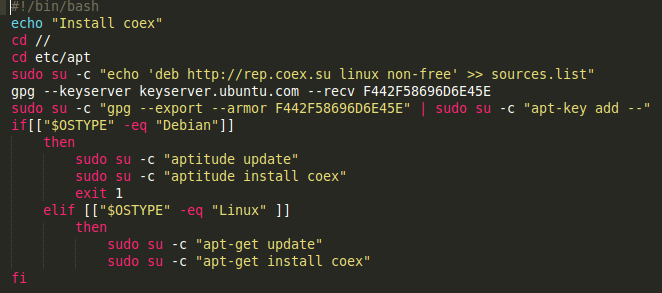
\includegraphics[width=0.7\linewidth]{ser_1}}
\caption{ Программа для внесения изменений в sources.list }
\label{ser_1:ser_1}
\end{figure}

Изменения включают в себя адрес до репозитория   в сети Internet, где хранится deb пакет программного комплекса <<COEX>>, а также запись ключа, которым подписывают скаченные файлы с репозитория, вносятся также команды по установки и обновлению пакета при скачивании через менеджера. Данные действия позволяет менеджеру обновлений операционной системы Linux следить за версиями deb пакета в репозиторие, содержащего программный комплекс <<COEX>>, при появление новой версии менеджер сообщит пользователю о возможном обновлении. Первая программа находится на сайте проекта <<COEX>>, скачивается и запускается пользователем. 

Вторая программа находится на сервере с репозиториям, и с помощью системной утилиты CRON запускается в определенное время, при наличии изменений из ветки master в системе контроля версий git (рисунок~\ref{ser_2:ser_2}).

\begin{figure}[!ht]
\center{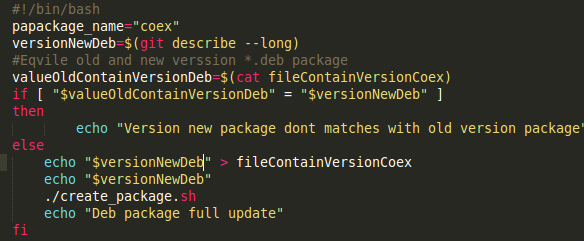
\includegraphics[width=0.7\linewidth]{ser_2}}
\caption{ Программа  для запуска сборки по времени  с помощью демона  «CRON» }
\label{ser_2:ser_2}
\end{figure}

Скрипт-программа на основе сведений из системы контроля версий GIT проекта <<COEX>>, создает версию для двоичного пакета формата deb, сам deb пакет создается при помощи скрипт-программы по созданию  deb пакета из тексты программ проекта (рисунок~\ref{ser_3:ser_3}).

\begin{figure}[!ht]
\center{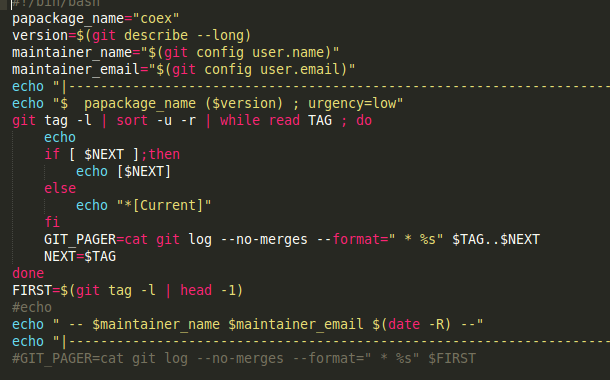
\includegraphics[width=0.7\linewidth]{ser_3}}
\caption{ Программа для присвоения версии }
\label{ser_3:ser_3}
\end{figure}

Тестирование проводилось, на операционной системе «Debian 8.4», и ее наследниках(Ubuntu(16.04), Mint (17.3))(рисунки~\ref{ser_4:ser_4}-~\ref{ser_6:ser_6}).

\begin{figure}[!ht]
\center{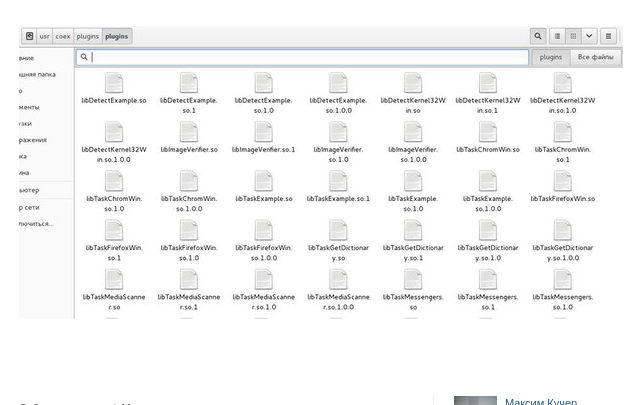
\includegraphics[width=0.7\linewidth]{ser_4}}
\caption{ Установка на Debian }
\label{ser_4:ser_4}
\end{figure}

\begin{figure}[!ht]
\center{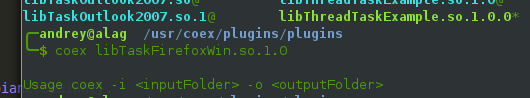
\includegraphics[width=0.7\linewidth]{ser_5}}
\caption{ Установка на Mint }
\label{ser_5:ser_5}
\end{figure}

\begin{figure}[!ht]
\center{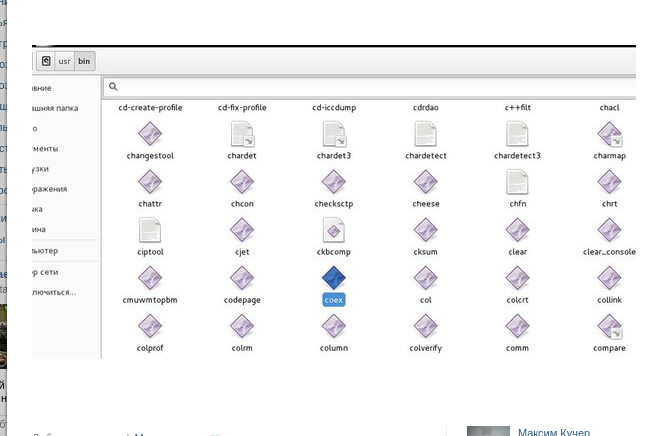
\includegraphics[width=0.7\linewidth]{ser_6}}
\caption{ Установка на Ubuntu }
\label{ser_6:ser_6}
\end{figure}

В ходе тестирования проверялось корректность работы двоичного пакета после прохождения автоматизированной сборки, также проверялась функционирование программного комплекса <<COEX>>, и корректность удаления проекта с компьютера пользователя. Результатом тестирования были выявлены проблемы с некаторами зависимостями модулей, и связи модулей c программным ядром <<COEX>>. После выявления проблем были перепроверены и исправлены зависимости, в модулях где были найдены ошибки с зависимостями. А также переделана структура пакета, для исправления проблемы взаимодействия ядра <<COEX>> и его модулей при установке через двоичный пакет.  

\clearpage


%  % ---------Отчет Олега---------------%
\newpage 
\subsection{Доработка сайта проекта <<COEX>>}
В прошлом семестре была начата разработка веб-сайта, представляющего программный комплекс COEX интернету. Была создана главная страница и небольшое наполнение контентом. На данный семестр были поставлены следующие задачи:

\begin{itemize}
  \item исправление дизайна;
  \item добавление вывода новостей;
  \item актуализация информации, представленной на сайте.
\end{itemize}

\subsubsection{Исправление дизайна и актуализация информации}

Для новых плагинов созданы иконки (рис.~\ref{lob_1:lob_1}).

\begin{figure}[h!]
\center{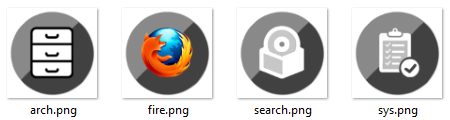
\includegraphics[width=0.8\linewidth]{lob_1}}
\caption{Иконки модулей}
\label{lob_1:lob_1}
\end{figure}

Общая архитектурная схема системы из изображения была свёрстана в HTML + CSS код (рис.~\ref{lob_2:lob_2} и~\ref{lob_3:lob_3}).

\begin{figure}[h!]
\center{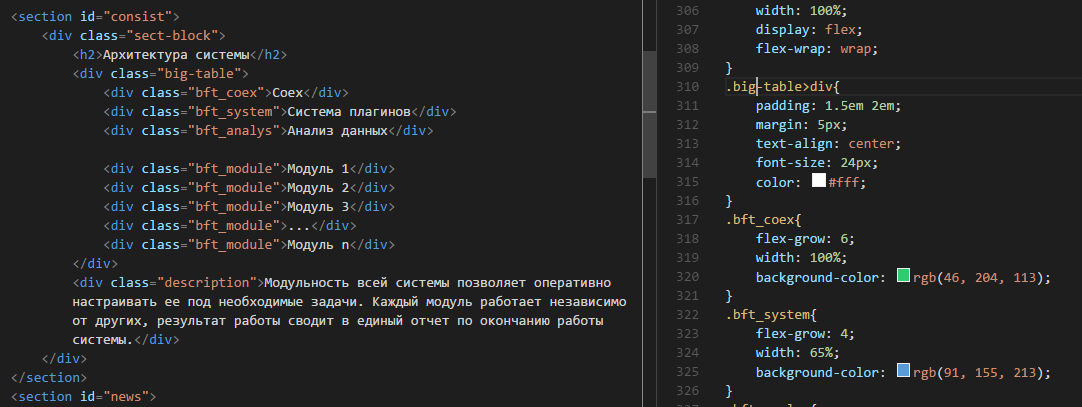
\includegraphics[width=1\linewidth]{lob_2}}
\caption{HTML + CSS код блока схемы системы}
\label{lob_2:lob_2}
\end{figure}

\begin{figure}[h!]
\center{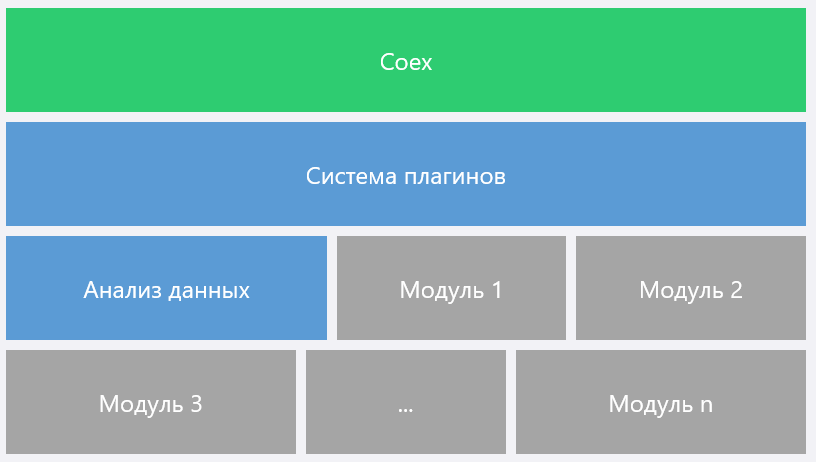
\includegraphics[width=1\linewidth]{lob_3}}
\caption{Схема системы}
\label{lob_3:lob_3}
\end{figure}

Доработана нижняя часть сайта (футер), представленный на рисунке~\ref{lob_4:lob_4}.

\begin{figure}[h!]
\center{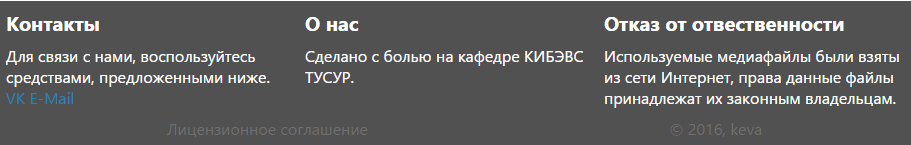
\includegraphics[width=1\linewidth]{lob_4}}
\caption{Футер сайта}
\label{lob_4:lob_4}
\end{figure}

\subsubsection{Добавление вывода новостей}

Создана группа в социальной сети Вконтакте, где в дальнейшем будут выкладывать новости проекта (рис.~\ref{lob_5:lob_5}).

\begin{figure}[h!]
\center{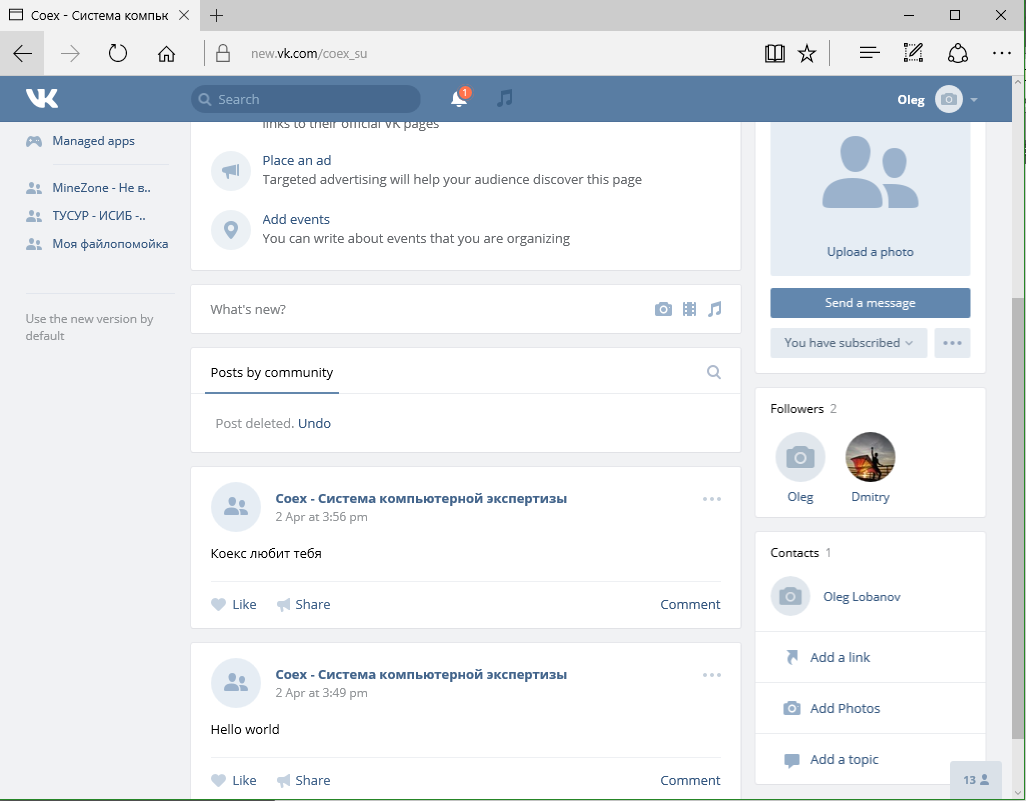
\includegraphics[width=1\linewidth]{lob_5}}
\caption{Группа проекта в ВК}
\label{lob_5:lob_5}
\end{figure}

Используя API, предоставляемый социальной сетью Вконтакте, был сгенерирован виджет новостей проекта для сайта (рис.~\ref{lob_6:lob_6} и~\ref{lob_7:lob_7}).

\begin{figure}[h!]
\center{\includegraphics[width=0.7\linewidth]{lob_6}}
\caption{Код виджета}
\label{lob_6:lob_6}
\end{figure}

\begin{figure}[h!]
\center{\includegraphics[width=1\linewidth]{lob_7}}
\caption{Новости на сайте}
\label{lob_7:lob_7}
\end{figure}

\clearpage
	

\newpage
\subsection{Разработка плагина PDFChecker}
Стандарт PDF начиная с версии 1.3, введенный компанией Adobe \cite{adobe}, предусматривает возможность использования интерактивных элементов внутри документа, в том числе созданных с использованием сценарного языка программирования JavaScript. Такую возможность часто используют для сокрытия какой-либо информации или дополнительного функционала, которые при беглом просмотре могут быть незаметны. 

Исходя из этого встал вопрос о поиске таких <<подозрительных>> файлов в исследуемой системе.

Задание: написать плагин, который будет находить PDF документы со встроенными JavaScript сценариями (рис.~\ref{lob_8:lob_8}).

\begin{figure}[h!]
\center{\includegraphics[width=1\linewidth]{lob_8}}
\caption{Вырезка из стандарта PDF 1.3}
\label{lob_8:lob_8}
\end{figure}

Согласно этому стандарту, все JavaScript сценарии обрамляются обязательным ключом <<JS>>, поэтому задача сводится к обнаружению этого ключа в заголовочном блоке PDF документа. Для этого был реализован алгоритм (представлен на рисунке~\ref{lob_9:lob_9}). Результат работы плагина можно увидеть на рисунке~\ref{lob_10:lob_10}.

\begin{figure}[h!]
\center{\includegraphics[width=0.8\linewidth]{lob_10}}
\caption{Результат работы плагина}
\label{lob_10:lob_10}
\end{figure}

\begin{figure}[h!]
\center{\includegraphics[width=0.8\linewidth]{lob_9}}
\caption{Алгоритм поиска JavaScript в PDF}
\label{lob_9:lob_9}
\end{figure}

\clearpage


 % ---------Отчет Ильи---------------%
\newpage
\subsection{Документирование плагинов}

На данный момент основной репозиторий находится на ресурсе GitHub. Данный ресурс использует язык разметки MarkDown (подробнее в разделе~\ref{sec:markdown}) и автоматически добавляет файл <<Readme.md>> к описанию программного модуля, если этот файл присутствует. В связи с этим было решено создать документацию плагинов, используя MarkDown. Документация должна включать в себя:

\begin{enumerate}
  \item Название плагина;
  \item Версию плагина;
  \item Автора плагина;
  \item Описание плагина;
  \item Требуемую операционную систему;
  \item Версию ПО, с которым этот плагин работает;
  \item Основные методы плагина с описанием входов и выходов.
\end{enumerate}

Результат разработанной документации можно наблюдать на странице плагина в репозитории (рис.~\ref{bok_1:bok_1}).

\begin{figure}[h!]
\center{\includegraphics[width=0.8\linewidth]{bok_1}}
\caption{ Документация в веб-интерфейсе репозитория }
\label{bok_1:bok_1}
\end{figure}

Поскольку проект <<COEX>> имеет свою собственную веб-страницу, данную документацию также необходимо преобразовать в формат HTML, чтобы затем добавить на веб-страницу проекта. Для преобразования был разработан небольшой скрипт на языке Python (приложение ~\ref{apx:mdtohtml}). На рисунке ~\ref{bok_2:bok_2} можно наблюдать ту же документацию, но в формате HTML.

\begin{figure}[h!]
\center{\includegraphics[width=0.9\linewidth]{bok_2}}
\caption{ Документация в формате HTML }
\label{bok_2:bok_2}
\end{figure}

\clearpage
\subsection{Разработка и внедрение копии жесткого диска}

Поскольку большое количество плагинов <<COEX>> обращается к жесткому диску для поиска тех или иных файлов, что в свою очередь создает серьезную нагрузку на него, то было решено модифицировать архитектуру проекта с целью хранения копии информации о жестком диске. Данную информацию решено было хранить как поле объекта <<config>>, к которому будут обращаться остальные плагины. Поле представляет из себя класс <<Hdd>> с атрибутом типа QList<QDir> (приложение ~\ref{apx:hddclass}). Данный тип был выбран, поскольку он позволяет хранить данные о всех директориях и файлах внутри них, а также предоставляет удобные интерфейсы для доступа к ним. Методы класса <<Hdd>>:

\begin{enumerate}
  \item Hdd::Hdd(QString path);
  \item Hdd::~Hdd();
  \item QFileInfoList getFiles(QStringList wildcardlist);
  \item QFileInfoList getFiles(QString wildcard).
\end{enumerate}

Метод <<Hdd::Hdd(QString path)>> является конструктором класса. Переменная <<path>>, подаваемая на вход метода является путем до начальной папки. Конструктор с помощью экземпляра класса <<QDirIterator>> посещает каждую папку в начальной папке и сохраняет данные о ней в переменную типа <<QDir>>, после чего добавляет эту переменную к массиву <<QList<QDir>>>, и наконец сохраняет полученный массив как поле класса. Алгоритм конструктора можно увидеть на рисунках~\ref{bok_6:bok_6} и~\ref{bok_7:bok_7}.

\begin{figure}[h!]
\center{\includegraphics[width=0.3\linewidth]{bok_6}}
\caption{ Алгоритм конструктора класса <<Hdd>> }
\label{bok_6:bok_6}
\end{figure}

\begin{figure}[h!]
\center{\includegraphics[width=0.5\linewidth]{bok_7}}
\caption{ Продолжение алгоритма конструктора класса <<Hdd>> }
\label{bok_7:bok_7}
\end{figure}

Метод <<Hdd::~Hdd()>> является деструктором класса.

Метод <<QFileInfoList getFiles(QStringList wildcardlist)>> возвращает объект <<QFileInfoList>> для всех файлов, которые соответствуют заданному массиву масок <<wildcardlist>>. Алгоритм метода можно увидеть на рисунке ~\ref{bok_9:bok_9}.

\begin{figure}[h!]
\center{\includegraphics[width=0.3\linewidth]{bok_9}}
\caption{ Алгоритм метода <<getFiles>> класса <<Hdd>> }
\label{bok_9:bok_9}
\end{figure}

Метод <<QFileInfoList getFiles(QString wildcard)>> выполняет ту же функцию, что и прошлый метод. Он является перегрузкой прошлого метода и принимает на вход одну маску вместо массива. Алгоритм метода можно увидеть на рисунке ~\ref{bok_8:bok_8}.

\begin{figure}[h!]
\center{\includegraphics[width=0.3\linewidth]{bok_8}}
\caption{ Алгоритм перегруженного метода <<getFiles>> класса <<Hdd>> }
\label{bok_8:bok_8}
\end{figure}

После разработки архитектуры класса, он был внедрен в <<скелет>> проекта. Класс конструируется перед работой плагинов, но после определения операционной системы.

\begin{figure}[h!]
\center{\includegraphics[width=1\linewidth]{bok_3}}
\caption{ Работа класса <<Hdd>> при запуске <<COEX>> }
\label{bok_3:bok_3}
\end{figure}

Далее необходимо было изменить плагины, таким образом, чтобы они обращались к сохраненной копии диска вместо самого диска. Таким образом были изменены два плагина - <<TaskMediaScanner>> и <<TaskChromeWin>>.

Теперь перед нами стояла задача сравнить нагрузку диска до и после внедрения класса <<Hdd>>. Поскольку нами использовался удаленный репозиторий и система контроля версий git, то это не составило проблемы по причине того, что разработка класса велась в отдельной <<ветке>>.

Было решено с помощью утилиты iotop замерить использование жесткого диска (в КБ/с) несколько раз до и после введения нового плагина и отфильтровать полученные результаты, чтобы учитывать исключительно нагрузку, создаваемую программой <<COEX>>. Для этого был разработан мультипоточный скрипт на языке Python, запускающий отдельно утилиту <<iotop>> и <<COEX>> и фильтрующий результаты, сохраняемые утилитой <<iotop>> (приложение ~\ref{apx:diskusage}):

\begin{figure}[h!]
\center{\includegraphics[width=1\linewidth]{bok_4}}
\caption{ Результат работы скрипта }
\label{bok_4:bok_4}
\end{figure}

Далее результаты были обработаны, и на основании их был построен график, показывающий нагрузку на жесткий диск до и после внедрения класса <<Hdd>>. Было решено оставить по 10 итераций на каждое измерение, поскольку после этого количества разница между итерациями была минимальна и уже прослеживалась значимая разница между измерениями.

\begin{figure}[h!]
\center{\includegraphics[width=1\linewidth]{bok_5}}
\caption{ Сравнение нагрузки на жесткий диск до и после изменения архитектуры }
\label{bok_5:bok_5}
\end{figure}

Из графика видно, что даже при изменении всего двух плагинов для использования новой архитектуры нагрузка на диск заметно снизилась. Так как на данный момент в проекте <<COEX>> имеется 17 рабочих плагинов, преобразование каждого из них должно сильно сказаться на нагрузке жесткого диска в лучшую сторону.

\clearpage


 % ---------Отчет Марины--------------%
\newpage
\subsection{Многопоточное программирование} 
Одной из поставленных в данном семестре задач стало изучение возможностей многопоточного программирования с использованием программной библиотеки Qt. Программирование потоков осуществляется с помощью класса QThreads, а также механизма сигналов и слотов.

Все это необходимо для того, чтобы реализовать в системе <<COEX>> параллельное выполнение программных модулей (<<плагинов>>), осуществляющих поиск остаточных данных с образа системы, изображений, различных файлов и т.д. 

\subsubsection{Сигналы и слоты}

Сигналы и слоты используются для связи между объектами. Механизм сигналов и слотов --- это основная особенность Qt и, вероятно, основная часть Qt, которая больше всего отличается по функциональности от других библиотек.

Более старые инструментарии обеспечивают подобную связь с помощью функций обратного вызова. Обратный вызов --- это указатель на функцию. Если необходимо, чтобы функция обработки уведомила о некотором событии, ей передается указатель на другую функцию (отзыв). Функция обработки вызовет функцию обратного вызова, когда это будет уместно. Но данный подход имеет два фундаментальных недостатка: во-первых, он не типобезопасен. Мы некогда не сможем проверить, что функция обработки вызывает отзыв с правильными аргументами. Во-вторых, этот метод жестко связан с функцией обработки, так как она должна знать, какой отзыв вызывать.

В Qt используется техника, альтернативная функциям обратного вызова: механизм сигналов и слотов. Сигнал испускается, когда происходит определенное событие. Слот --- это функция, вызываемая в ответ на определенный сигнал.

Этот механизм типобезопасен: сигнатура сигнала должна соответствовать сигнатуре принимающего слота (фактически, слот может иметь более короткую сигнатуру, чем сигнал, который он получает, поскольку может игнорировать лишние аргументы). Сигналы и слоты связаны нежёстко: класс, испускающий сигналы, не знает и не интересуется, который из слотов получит сигнал. Механизм сигналов и слотов Qt гарантирует, что, если сигнал соединен со слотом, слот будет вызываться с параметрами сигнала в нужный момент. Сигналы и слоты могут иметь любое количество аргументов любых типов. Они полностью типобезопасны.

Все классы, наследуемые от QObject или одного из его подклассов (например, QWidget) могут содержать сигналы и слоты. Сигналы испускаются при изменении объектом своего состояния, если это изменение может быть интересно другим объектам. Все объекты делают это для связи с другими объектами. Их не заботит, получает ли кто-нибудь испускаемые ими сигналы. Это является истинной инкапсуляцией информации, и она гарантирует, что объекты могут использоваться как отдельные компоненты программного обеспечения.

Слоты могут получать сигнал, но они также являются обыкновенными функциями-членами. Также, как объект не знает, получает ли кто-нибудь сигналы, испускаемые им, слоты не знают, существуют ли сигналы, с ними связанные. Это гарантирует, что можно создать полностью независимые Qt-компоненты.

Можно присоединять к одному слоту столько сигналов, сколько необходимо, и один сигнал может быть соединен со столькими слотами, сколько требуется. Также возможно соединение сигнала непосредственно с другим сигналом (второй сигнал будет испускаться немедленно всякий раз, когда испускается первый).

Вместе сигналы и слоты представляют собой мощный механизм компонентного программирования. Графическое представление связи сигналов и слотов различных объектов можно увидеть на рисунке~\ref{signals-slots:signals-slots}.

\textbf{тут ссылка на http://doc.crossplatform.ru/qt/4.3.2/signalsandslots.html}

\begin{figure}[h!]
\center{\includegraphics[width=0.8\linewidth]{signals-slots}}
\caption{ Механизм сигналов и слотов для связи объектов в Qt }
\label{signals-slots:signals-slots}
\end{figure}

\subsubsection{Потоки QThreads}

В многопоточных приложениях, обслуживание интерфейса производится в отдельном потоке, а обработка данных -- в другом (одном или нескольких) потоке. В результате приложение сохраняет возможность откликаться на действия пользователя даже во время интенсивной обработки данных. Еще одно преимущество многопоточности -- на многопроцессорных системах различные потоки могут выполняться на различных процессорах одновременно, что несомненно увеличивает скорость исполнения.

Для реализации потоков Qt предоставляет класс QThread.

Поток — это независимая задача, которая выполняется внутри процесса и разделяет вместе с ним общее адресное пространство, код и глобальные данные.

Процесс, сам по себе, не является исполнительной частью программы, поэтому для исполнения программного кода он должен иметь хотя бы один поток (далее -- основной поток). Конечно, можно создавать и более одного потока. Вновь созданные потоки начинают выполняться сразу же, параллельно с главным потоком, при этом их количество может изменяться — одни создаются, другие завершаются. Завершение основного потока приводит к завершению процесса, независимо от того, существуют другие потоки или нет.Создание нескольких потоков в процессе получило название многопоточность.

\textbf{http://qt-doc.ru/processy-i-potoki-v-qt.html}

Для использования многопоточности нужно унаследовать класс от QThread. Чтобы запустить поток, нужно вызвать метод start().

Каждый поток может иметь собственный цикл обработки событий. Главный поток начинает цикл обработки событий, используя QCoreApplication::exec(); другие потоки могут начать свои циклы обработки событий, используя QThread::exec().

Цикл обработки событий потока делает возможным использование потоком некоторых неграфических классов Qt, которые требуют наличия цикла обработки событий (такие как QTimer, QTcpSocket и QProcess). Это также даёт возможность соединить сигналы из любых потоков со слотами в определённом потоке (рис.~\ref{thread-cycle:thread-cycle}).

\begin{figure}[h!]
\center{\includegraphics[width=0.8\linewidth]{thread-cycle}}
\caption{ Цикл обработки событий потоков в Qt }
\label{thread-cycle:thread-cycle}
\end{figure}

\textbf{http://doc.crossplatform.ru/qt/4.4.3/threads.html}

Для того, чтобы запускать программные модули на выполнение в нескольких потоках и должным образом завершать их выполнение, понадобилось написать контроллер --- объект, который создает потоки для уже существующих объектов (самих плагинов), перемещает эти объекты в созданные потоки. Далее он запускает их выполнение при помощи метода Controller::start\_threads(). После того, как каждый поток завершается, он посылает сигнал контроллеру о завершении finished() и переходит в режим ожидания. Когда все потоки завершаются, контроллер задействует слот stop\_threads(), предназначенный для того, чтобы послать сигнал об успешном завершении работы как всех потоков, так и работы самого контроллера, основной программе. При этом для связи сигналов и слотов используется функция connect(object\_1, SIGNAL(signal\_1), object\_2, SLOT(slot\_2)).  

Поскольку главный поток (основная программа) начинает цикл обработки событий, используя QCoreApplication::exec(), при получении сигнала finished(), сгенерированного контроллером, цикл обработки событий главного потока прерывается и главная программа успешно завершается. 

Результат вывода программы представлен на рисунке~\ref{program-output:program-output}.

\begin{figure}[h!]
\center{\includegraphics[width=0.8\linewidth]{program-output}}
\caption{ Вывод программы qthreads }
\label{program-output:program-output}
\end{figure}

Кроме написания потокового контроллера был доработан плагин ThreadTaskICQ таким образом, чтобы учитывались особенности работы с механизмом сигналов и слотов. Только после этого плагин может быть запущен в потоке с использованием класса QThreads.  

\subsubsection{Итоги работы за семестр}

Таким образом, в течение семестра была написана рабочая программа-реализация многопоточного программирования с использованием программной кроссплатформенной библиотеки Qt. Изучены некоторые особенности работы механизма слотов и сигналов. Доработан модуль ThreadTaskICQ. В дальнейшем планируется имплементировать написанный контроллер потоков под архитектуру системы <<COEX>>, а также дописать должным образом плагины для реализации возможности выполнения программных модулей в потоках с использованием слотов и сигналов. 







\newpage
\section*{Заключение}
\addcontentsline{toc}{section}{Заключение}
В данном семестре нашей группой была выполнена часть работы по созданию автоматизированного программного комплекса для проведения компьютерной экспертизы. Основной целью в данном семестре стала подготовка проекта <<COEX>> к релизу, для чего были разработаны веб-сайт и репозиторий проекта, графический интерфейс пользователя, доработаны некоторые из программных модулей, собран <<бинарный>> пакет для установки и распространения системы <<COEX>>. 

Также написана рабочая программа-реализация для многопоточного выполнения программных модулей с использованием программной кроссплатформенной библиотеки Qt. Изучены некоторые особенности работы механизма слотов и сигналов. В дальнейшем планируется имплементировать написанный контроллер потоков под архитектуру системы <<COEX>>, а также дописать должным образом плагины для реализации возможности выполнения программных модулей в потоках с использованием механизма слотов и сигналов.
 
 
 \newpage
 \renewcommand{\refname}{Список использованных источников}
 \bibliography{lit}

 \ESKDappendix{Обязательное}{\normalfont Компакт-диск}
 Компакт-диск содержит: 
 \begin{itemize}
 \item электронную версию пояснительной записки в форматах *.tex и *.pdf;
 \item актуальную версию программного комплекса для проведения компьютерной экспертизы;
 \item тестовые данные для работы с программным комплексом.
 \end{itemize}
 
  \ESKDappendix{}{\normalfont Md to html script}\label{apx:mdtohtml}
\begin{lstlisting}
  
import markdown2
import os
import glob

def compose_anycase(string):
	result = ""
	for letter in string:
		result += "[%s%s]" % (letter.lower(), letter.upper())
	return result
		
path = os.path.join("sources", "plugins", "*")
readmes = glob.glob(os.path.join(path, compose_anycase("readme.md")))

for readme in readmes:
	outpath = "%s%s%s" % (os.path.dirname(readme), os.sep, "Readme.html")
	with open(outpath, 'w') as outfile, open(readme, 'r') as infile:
		file = infile.read()
		html = markdown2.markdown(file).encode('utf-8')
		outfile.write(html)
\end{lstlisting}

 
 \ESKDappendix{}{\normalfont Hdd class}\label{apx:hddclass}
\begin{lstlisting}
#include "hdd.h"
#include <QDebug>

Hdd::Hdd(QString path){
    QDirIterator dirPath(path, QDir::Dirs | QDir::NoSymLinks 
      | QDir::Hidden, QDirIterator::Subdirectories);
    QList<QDir> dirList;

    while (dirPath.hasNext())
    {
        QDir directory(dirPath.next());
        if (!dirList.contains(directory))
        {
            dirList.append(directory);
        }
    }

    this->infoList = dirList;

    //debug
    /*
    QFile file("/home/ventar/test/test.txt");
    QStringList wildcard = (QStringList() << "*.jpg");
    if (file.open(QIODevice::WriteOnly))
    {
        foreach(QDir directory, this->infoList)
        {
            QTextStream stream(&file);
            stream << directory.absolutePath() << endl;
            QFileInfoList list = directory.entryInfoList(QDir::Files 
              | QDir::NoSymLinks | QDir::Hidden);
            foreach (QFileInfo fileInfo, list)
            {
                stream << fileInfo.absoluteFilePath() << endl;
            }
        }
    }
    */
}

Hdd::~Hdd(){

}

QFileInfoList Hdd::getFiles(QStringList wildcardlist){

    QFileInfoList allists;
    foreach(QDir dir, Hdd::infoList){
        allists.append(dir.entryInfoList( wildcardlist, QDir::Files  
          | QDir::NoSymLinks | QDir::Hidden ));
    }

    return allists;
}

QFileInfoList Hdd::getFiles(QString wildcard){

    QStringList wildcardlist;
    wildcardlist.append(wildcard);
    return Hdd::getFiles(wildcardlist);
}
\end{lstlisting}

  
 \ESKDappendix{}{\normalfont Disk usage logging script}\label{apx:diskusage}
\begin{lstlisting}
import os
import sys
from threading import Thread

class IotopThread(Thread):
    def __init__(self):
        Thread.__init__(self, target=self.main)
        self.daemon = True
        self.time = 300
    def main(self):
        print "Starting 'iotop'"
        os.system("iotop -botqqqk --iter={0} 
          >> /var/log/iotop".format(self.time))
        
        sys.exit()
        
class TestPlugin(Thread):
    def __init__(self):
        Thread.__init__(self, target=self.main)
        self.daemon = True
    def main(self):
        print "Starting 'testplugin.sh'"
        os.system("/home/ventar/coex/test.sh")
        
        sys.exit()
        
io_thread = IotopThread()
plugin_thread = TestPlugin()
io_thread.start()
plugin_thread.start()
while (io_thread.isAlive() or plugin_thread.isAlive()):
    pass
with open("/var/log/iotop", "r") as infile:
    file = infile.read()
lines = file.split("\n")
lines = [x for x in lines if "coex" in x]
with open ("/home/ventar/result.txt", "w") as outfile:
    for line in lines:
        print line
        outfile.write(line + "\n")
\end{lstlisting}

 
\end{document}
